
\section{Introduction}

The two-phase optimisation via simulation of healthcare Emergency
Departments, ED, proposed in \ref{ch3:Proposed-OvS-ED} was applied
herewith to analyse the administrative strategies leading to optimum
decisions about the physical and human resources of an ED. In particular,
the impact on the economics and the productivity of Sabadell Hospital
ED of different sanitary staff configuration (v.gr., doctors, triage
nurses, admission personnel, emergency nurses, and x-ray technicians)
were analysed. It is a discrete combinatorial optimisation problem.

There are three main issues to be addressed to carry out the evaluation,
namely: the \textit{simulation models} that represent the system under
study (discussed along the previous chapters); the \textit{decision
variables} and\textit{ workloads} used as inputs of the simulation
models; and the \textit{metrics} used to asses the benefits of the
proposal. We have defined some significant workloads and a set of
metrics to observe both functional and performance features of the
proposal. This set of metrics were defined in term of three different
indexes, namely: patient length of stay (LoS) in the ED; number of
attended patients per day (Throughput); and a compound index, the
product of the cost of a given sanitary staff configuration times
patient length of stay (CLoS).

In the following sections, the \textit{decision variables, }the\textit{
workloads}, and the \textit{metrics} are described. Finally two case
scenarios and their results are presented and discussed. 


\section{Field Information of Sabadell Hospital ED}

It was found through interviews with the managers at the EDs of Sabadell
hospital (which provides healthcare services to an average of 160,000
patients/year), it was found that a basic sanitary of its ED staff
is composed by: doctors, triage nurses, emergency nurses, admission
personnel, and x-ray technicians, as shown in \ref{tab:T1}. This
table also shows some characteristics of such sanitary staff, namely:
sort of staff as junior or senior (that represents less and more expertise,
respectively); their respective costs (� \textbf{}%
\footnote{\textbf{It is not an actual euro, could be any currency.\label{fn:euro}}%
}); the operational patient-service-time (hours); and the minimum and
maximum number of each kind of staff. 

\begin{comment}
 %
\saveFN\mymark  %
\end{comment}
\foreignlanguage{american}{}%
\begin{comment}
 %
\useFN\mymark  %
\end{comment}


\begin{table}[H]
\caption{Sabadell Hospital ED staff and their: associated expertise, costs,
operational patient-service time, and number.}


\begin{centering}
\begin{tabular}{>{\centering}m{3.5cm}>{\centering}p{1.1cm}>{\centering}p{1cm}>{\centering}p{1.1cm}>{\centering}p{1cm}>{\centering}m{0.075cm}>{\centering}m{2.2cm}}
\cline{1-5} \cline{7-7} 
\multicolumn{1}{>{\centering}m{3.5cm}|}{\textbf{Sanitary staff} } & \multicolumn{2}{c|}{\textbf{Cost (�$^{1}$)}} & \multicolumn{2}{c}{\textbf{Time/patient (hours)}} &  & \textbf{Number of personnel}\tabularnewline
\cline{1-5} \cline{7-7} 
 & Senior  & Junior  & Senior & Junior &  & min - Max\tabularnewline
\cline{1-5} \cline{7-7} 
Doctor  & 1000  & 500  & 0.26 & 0.35 &  & \textbf{\textit{1 -- 4}} \tabularnewline
\cline{1-5} \cline{7-7} 
Triage Nurse  & 500  & 350  & 0.09 & 0.13 &  & \textbf{\textit{1 -- 3}} \tabularnewline
\cline{1-5} \cline{7-7} 
Emergency Nurse & 500  & 350  & 0.14 & 0.18 &  & \textbf{\textit{1 -- 2}} \tabularnewline
\cline{1-5} \cline{7-7} 
Admission personnel & 200  & 150  & 0.02 & 0.035 &  & \textbf{\textit{1 -- 3}} \tabularnewline
\cline{1-5} \cline{7-7} 
X-ray technician & 200  & 150  & 0.09 & 0.14 &  & \textbf{\textit{1 -- 2}} \tabularnewline
\cline{1-5} \cline{7-7} 
\end{tabular}
\par\end{centering}

\label{tab:T1} 
\end{table}


\begin{figure}[H]
\centering 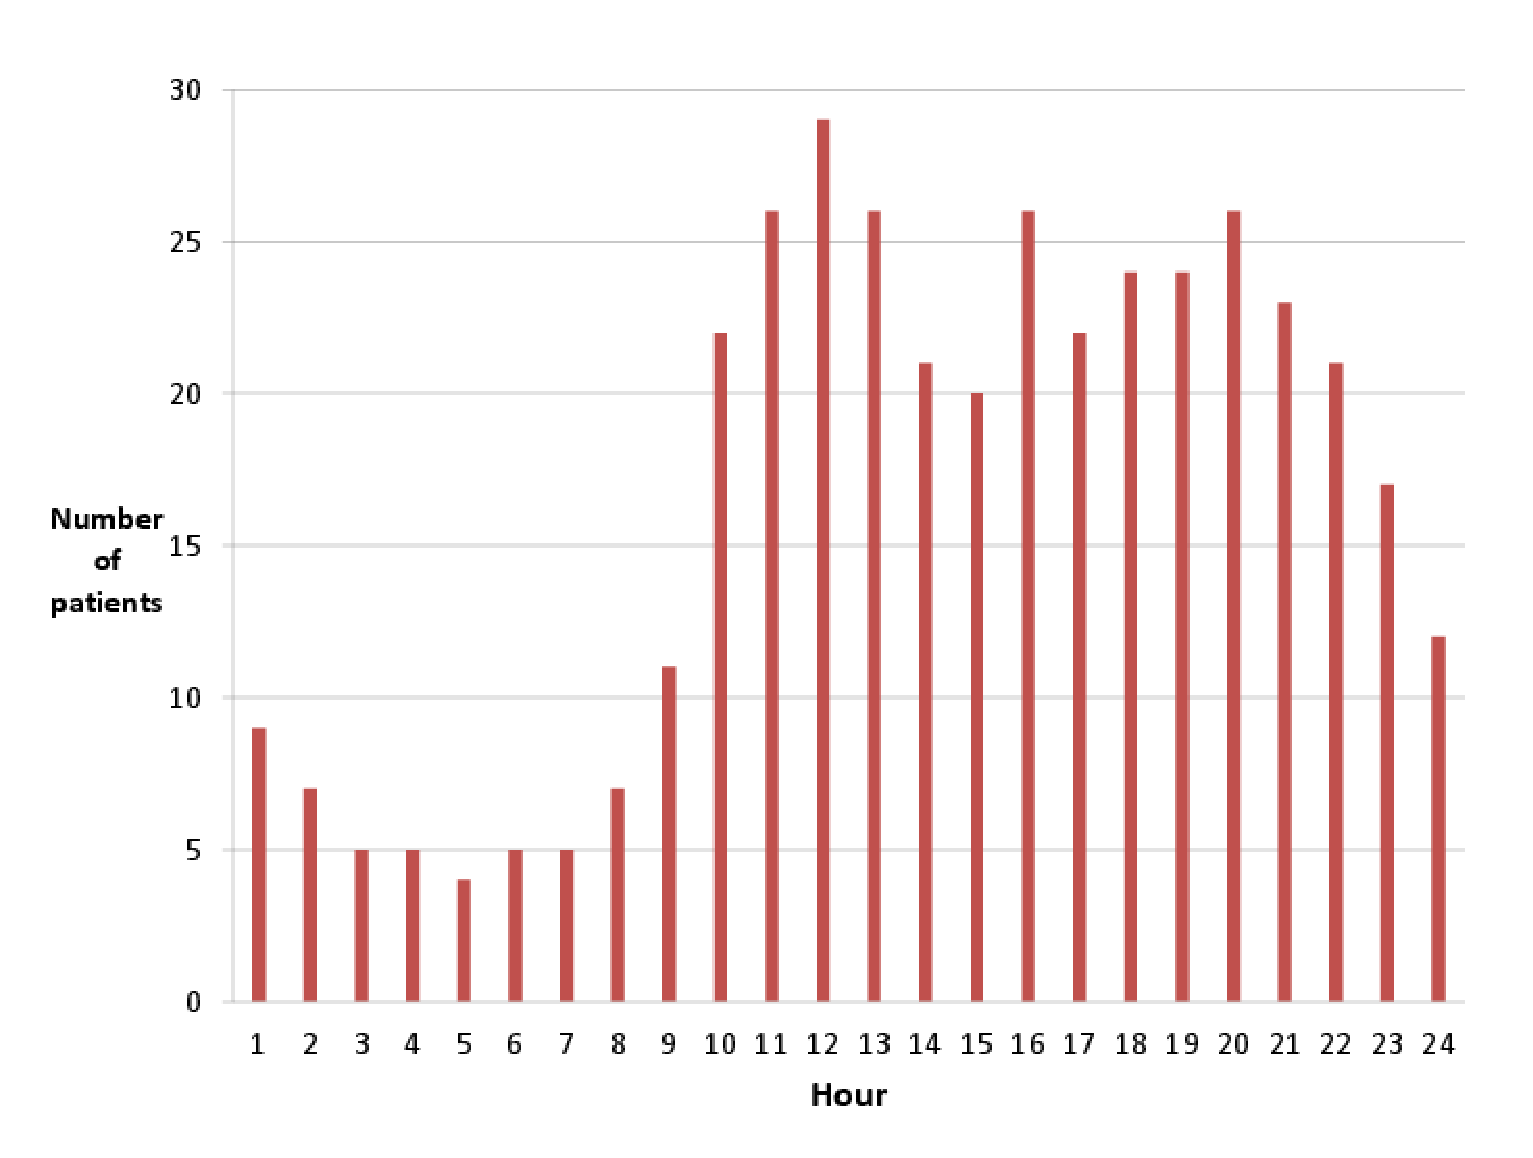
\includegraphics[width=0.85\columnwidth,height=0.17\paperheight]{figs4/input} 

\caption{Sabadell Hospital ED average of 400 daily incoming patients and its
hourly distribution (February 2010).\label{fig:real-input}}
\end{figure}


In reference to the Sabadell Hospital ED incoming patients, an average
of four hundred of patients daily arrive to the ED of Sabadell hospital.
As example, the statistics corresponding to February 2010, of this
real average number of incoming patients and its hourly distribution
are shown in \ref{fig:real-input}. As stated in \ref{sec:active-agents}
all incomings patients are triaged to identify the acuity of them
and to prioritise their urgency of attention. Thus, the average percentage,
according to the priority level of urgency of attention, of the incoming
patients to the ED of Sabadell hospital is as follows: triage level
1 - 1\%; triage level 2 - 4\%; triage level 3 - 20\%; triage level
4 - 32\%;and triage level 5 - 43\%. Patients identified as triage
level 4 and triage level 5 represent up to 75\% of the total of the
incoming patients to the ED of Sabadell hospital.

\begin{comment}
All simulations were done using the simulator previously explained,
utilising the \emph{BehaviorSpace} tool, serially and using the cluster
\textit{IBM} of the department, which has 32 Compute nodes with 2
x Dual-Core Intel(R) Xeon(R) CPU 5160 running at 3.00GHz, with 12
GB of RAM, and 4MB of L2 share cache (2x2)
\end{comment}


%\begin{figure}[htb!] 
%\centering 
%\begin{tabular}{ccc} 	
%	\subfloat[][9 Admission (A) personnel staff cases. AD\textit{i} represents Admission Den %\textit{i}.] 
%{\label{subfloat:adm_comb} 
%\resizebox{1.7in}{!} { 
%\begin{tabular}{cccc} 
%\hline 
%Case number & \bf{AD$_1$} & \bf {AD$_2$}  & \bf {AD$_3$}  \\ \hline 
%1 & AS  & -  & -    \\ \hline 
%2 & AJ  & -  & -    \\ \hline 
%3 & AS  & AS  & -    \\ \hline 
%4 & AJ  & AJ  & -    \\ \hline 
%5 & AS  & AJ  & -    \\ \hline 
%6 & AS  & AS  & AS    \\ \hline 
%7 & AJ  & AJ  & AJ    \\ \hline 
%8 & AS  & AJ  & AJ    \\ \hline 
%9 & AS  & AS  & AJ    \\ \hline 
%\end{tabular} 
%}         
%} 
%& 	
%	\subfloat[][9 Nurse (N) cases. TR\textit{i} represents Triage Room \textit{i}.] 
%{\label{subfloat:nur_comb} 
%\resizebox{1.7in}{!} { 
%\begin{tabular}{cccc} 
%\hline 
%Case number & \bf {TR$_1$} & \bf {TR$_2$}  & \bf {TR$_3$}  \\ \hline 
%1 & NS  & -  & -    \\ \hline 
%2 & NJ  & -  & -    \\ \hline 
%3 & NS  & NS  & -   \\ \hline 
%4 & NJ  & NJ  & -   \\ \hline 
%5 & NS  & NJ  & -   \\ \hline 
%6 & NS  & NS  & NS  \\ \hline 
%7 & NJ  & NJ  & NJ  \\ \hline 
%8 & NS  & NJ  & NJ  \\ \hline 
%9 & NS  & NS  & NJ  \\ \hline 
%\end{tabular} 
%}         
%} 
%&         
%	\subfloat[][14 Doctor (D) cases.  DR\textit{i} represents Diagnosis Room \textit{i}.] 
%{\label{subfloat:doc_comb} 
%\resizebox{1.99in}{!} {
%\begin{tabular}{ccccc} 
%\hline 
%Case number & \bf {DR$_1$} & \bf {DR$_2$}  & \bf {DR$_3$}  & \bf {DR$_4$}  \\ \hline 
%1 & DS  & -  & -  & -  \\ \hline 
%2 & DJ  & -  & -  & -  \\ \hline 
%3 & DS  & DS  & -  & -  \\ \hline 
%4 & DJ  & DJ  & -  & -  \\ \hline 
%5 & DS  & DJ  & -  & -  \\ \hline 
%6 & DS  & DS  & DS  & -  \\ \hline 
%7 & DJ  & DJ  & DJ  & -  \\ \hline 
%8 & DS  & DJ  & DJ  & -  \\ \hline 
%9 & DS  & DS  & DJ  & -  \\ \hline 
%10 & DS  & DS  & DS  & DS  \\ \hline 
%11 & DJ  & DJ  & DJ  & DJ  \\ \hline 
%12 & DS  & DJ  & DJ  & DJ  \\ \hline 
%13 & DS  & DS  & DJ  & DJ  \\ \hline 
%14 & DS  & DS  & DS  & DJ  \\ \hline 
%\end{tabular} 
%}       
% } 
%\end{tabular} 
%\caption{Combinations of sanitary staff: Admission (A) personnel, Nurses (N) and Doctors (D). Two levels of expertise: Junior (J), and Senior (S).} 
%\label{fig:combs} 
%\end{figure} 



\section{Decision Variables of Sabadell Hospital ED}

The sanitary staff included in \ref{tab:T1} are the \textit{decision
variables} of the ED. 
\begin{table}[H]
\noindent \begin{centering}
\hfill{}%
\begin{minipage}[t]{0.45\columnwidth}%
\centering\resizebox{2.3in}{!}{%%
\begin{tabular}{>{\centering}m{1.4cm}>{\centering}m{1.2cm}>{\centering}m{1.2cm}>{\centering}m{1.2cm}}
\hline 
Case number & \textbf{AD\textsubscript{1} } & \textbf{AD\textsubscript{2}} & \textbf{AD\textsubscript{3}}\tabularnewline
\hline 
1 & AS & - & -\tabularnewline
2 & AJ & - & -\tabularnewline
3 & AS & AS & -\tabularnewline
4 & AJ & AJ & -\tabularnewline
5 & AS & AJ & -\tabularnewline
6 & AS & AS & AS\tabularnewline
7 & AJ & AJ & AJ\tabularnewline
8 & AS & AJ & AJ\tabularnewline
9 & AS & AS & AJ\tabularnewline
\hline 
\end{tabular}}

\caption{9 Admission (A) personnel cases. AD\textit{\textsubscript{\textit{i}}}
is Admission Den\textit{\textsubscript{\textit{i}}}.$\,$Where AJ
means Admission personnel Junior, whereas AS means Admission personnel
Senior. \label{subtab:As}}
%
\end{minipage}\hfill{}%
\begin{minipage}[t]{0.45\columnwidth}%
\centering\resizebox{2.3in}{!}{%%
\begin{tabular}{>{\centering}m{1.4cm}>{\centering}m{1.2cm}>{\centering}m{1.2cm}>{\centering}m{1.2cm}}
\hline 
Case number & \textbf{TR\textsubscript{1}} & \textbf{TR\textsubscript{2}} & \textbf{TR\textsubscript{3}}\tabularnewline
\hline 
1 & NS & - & -\tabularnewline
2 & NJ & - & -\tabularnewline
3 & NS & NS & -\tabularnewline
4 & NJ & NJ & -\tabularnewline
5 & NS & NJ & -\tabularnewline
6 & NS & NS & NS\tabularnewline
7 & NJ & NJ & NJ\tabularnewline
8 & NS & NJ & NJ\tabularnewline
9 & NS & NS & NJ\tabularnewline
\hline 
\end{tabular}}

\caption{9 Nurse (N) cases. TR\textit{\textsubscript{\textit{i}}} represents
Triage Room \emph{i}. Where NJ means Triage Nurse Junior, whereas
NS means Triage Nurse Senior.\foreignlanguage{american}{\label{subtab:Ns}}}
%
\end{minipage}\hfill{}\vspace{0.1cm}

\par\end{centering}

\noindent \centering{}\hfill{}%
\begin{minipage}[t]{0.45\columnwidth}%
\centering\resizebox{1.7in}{!}{%
\begin{tabular}{>{\centering}m{1.4cm}>{\centering}m{1.4cm}>{\centering}m{1.4cm}}
\hline 
Case number & \textbf{ENR\textsubscript{1} } & \textbf{ENR\textsubscript{2}}\tabularnewline
\hline 
1 & ENS & -\tabularnewline
2 & ENJ & -\tabularnewline
3 & ENS & ENS\tabularnewline
4 & ENJ & ENJ\tabularnewline
5 & ENS & ENJ\tabularnewline
\hline 
\end{tabular}}

\caption{5 Emergency nurse (EN) cases. EN\textit{R\textsubscript{\textit{i}}}
represents ENurse Room \emph{i}. Where ENJ means Emergency Nurse Junior,
whereas ENS means Emergency Nurse Senior\foreignlanguage{american}{\label{subtab:ENs}}}
%
\end{minipage}\hfill{}%
\begin{minipage}[t]{0.45\columnwidth}%
\centering\resizebox{1.7in}{!}{%%
\begin{tabular}{>{\centering}m{1.4cm}>{\centering}m{1.4cm}>{\centering}m{1.4cm}}
\hline 
Case number & \textbf{XR\textsubscript{1}} & \textbf{XR\textsubscript{2}}\tabularnewline
\hline 
1 & XRS & -\tabularnewline
2 & XRJ & -\tabularnewline
3 & XRS & XRS\tabularnewline
4 & XRJ & XRJ\tabularnewline
5 & XRS & XRJ\tabularnewline
\hline 
\end{tabular}}

\caption{5 X-ray technician (XR) cases. XR\textit{\textsubscript{\textit{i}}}
represents X-ray Room \emph{i}. Where XRJ means X-ray technician Junior,
whereas XRS means X-ray technician Senior\foreignlanguage{american}{\label{subtab:Xrs}}}
%
\end{minipage}\hfill{}
\end{table}
 The disaggregation of \ref{tab:T1} yields \ref{subtab:As}, which
includes 9 possible combinations of admission personnel (junior/senior);
\ref{subtab:Ns}, which also includes 9 possible combinations of triage
nurses (junior/senior); \ref{subtab:ENs}, that presents the 5 possible
combinations of emergency nurse (junior/senior); \ref{subtab:Xrs}
that shows the 5 possible combinations of x-ray technician (junior/senior);
and \ref{subtab:Ds}, with 14 possible combinations of doctors (junior/senior)
in which the examined cases for each type of staff were included.
It is a discrete combinatorial problem.

 %
\begin{table}[H]
\caption{  %
14 Doctor (D) cases. DR\textit{\textsubscript{\textit{i}}} represents
Diagnosis Room \emph{i}. Where DJ means Doctor Junior, whereas DS
means Doctor Senior\foreignlanguage{american}{.\label{subtab:Ds}} %
}
\centering\resizebox{2.6in}{!}{%%
\begin{tabular}{>{\centering}m{1.4cm}>{\centering}m{1.1cm}>{\centering}m{1.1cm}>{\centering}m{1.1cm}>{\centering}m{1.1cm}}
\hline 
  %
Case number %
 &   %
\textbf{DR\textsubscript{1}} %
 &   %
\textbf{DR\textsubscript{2} } %
 &   %
\textbf{DR\textsubscript{3}} %
 &   %
\textbf{DR\textsubscript{4}} %
\tabularnewline
\hline 
  %
1 %
 &   %
DS %
 &   %
- %
 &   %
- %
 &   %
- %
\tabularnewline
  %
2 %
 &   %
DJ %
 &   %
- %
 &   %
- %
 &   %
- %
\tabularnewline
  %
3 %
 &   %
DS %
 &   %
DS %
 &   %
- %
 &   %
- %
\tabularnewline
  %
4 %
 &   %
DJ %
 &   %
DJ %
 &   %
- %
 &   %
- %
\tabularnewline
  %
5 %
 &   %
DS %
 &   %
DJ %
 &   %
- %
 &   %
- %
\tabularnewline
  %
6 %
 &   %
DS %
 &   %
DS %
 &   %
DS %
 &   %
- %
\tabularnewline
  %
7 %
 &   %
DJ %
 &   %
DJ %
 &   %
DJ %
 &   %
- %
\tabularnewline
  %
8 %
 &   %
DS %
 &   %
DJ %
 &   %
DJ %
 &   %
- %
\tabularnewline
  %
9 %
 &   %
DS %
 &   %
DS %
 &   %
DJ %
 &   %
- %
\tabularnewline
  %
10 %
 &   %
DS %
 &   %
DS %
 &   %
DS %
 &   %
DS %
\tabularnewline
  %
11 %
 &   %
DJ %
 &   %
DJ %
 &   %
DJ %
 &   %
DJ %
\tabularnewline
  %
12 %
 &   %
DS %
 &   %
DJ %
 &   %
DJ %
 &   %
DJ %
\tabularnewline
  %
13 %
 &   %
DS %
 &   %
DS %
 &   %
DJ %
 &   %
DJ %
\tabularnewline
  %
14 %
 &   %
DS %
 &   %
DS %
 &   %
DS %
 &   %
DJ %
\tabularnewline
\hline 
\end{tabular}}
\end{table}


  %
\ref{subtab:As} to \ref{subtab:Ds} were ordered by the sort and
number of staff, whereas \ref{subtab:As-pipe} to \ref{subtab:XRs-pipe}
were ordered by the equivalent operational patient-service time \foreignlanguage{american}{(t{*})}
of a ``single one'' sanitary professional (working in parallel)
of each sanitary staff configuration (admission personnel, nurses,
doctors, and x-ray technicians). This order was obtained by applying
the pipeline scheme described in \ref{sub:Pipeline-Model-ED} and
is graphically shown in \ref{fig:3D-scattered-LoS-wo} to \ref{fig:3D-scattered-LoS-tpipe}.
In these figures the index value was represented by colours, the most
important values in such figures were the green ones. 
\begin{table}[h]
 %
\caption{  %
Ordering staff configuration of admission personnel according to the
equivalent operational patient-service time \foreignlanguage{american}{(t{*})}
of each staff configuration.\label{subtab:As-pipe} %
}
\centering\resizebox{4.5in}{!}{%%
\begin{tabular}{>{\centering}m{1.4cm}>{\centering}m{1.4cm}>{\centering}m{1.2cm}>{\centering}m{1.2cm}>{\centering}m{1.2cm}>{\centering}m{1.2cm}>{\centering}m{1.2cm}>{\centering}m{1.2cm}}
\hline 
  %
Case number (t{*}) %
 &   %
Old case number %
 &   %
\textbf{AD\textsubscript{1} } %
 &   %
\textbf{AD\textsubscript{2}} %
 &   %
\textbf{AD\textsubscript{3}} %
 &   %
\textbf{�} %
 &   %
\textbf{Time (hrs)} %
 &   %
\textbf{t{*}}

\textbf{(hrs)} %
\tabularnewline
\hline 
  %
1 %
 &   %
6 %
 &   %
AS %
 &   %
AS %
 &   %
AS %
 &   %
600 %
 &   %
0.02 %
 &   %
0.007 %
\tabularnewline
  %
2 %
 &   %
9 %
 &   %
AS %
 &   %
AS %
 &   %
AJ %
 &   %
550 %
 &   %
0.035 %
 &   %
0.008 %
\tabularnewline
  %
3 %
 &   %
8 %
 &   %
AS %
 &   %
AJ %
 &   %
AJ %
 &   %
500 %
 &   %
0.035 %
 &   %
0.009 %
\tabularnewline
  %
4 %
 &   %
3 %
 &   %
AS %
 &   %
AS %
 &   %
- %
 &   %
400 %
 &   %
0.02 %
 &   %
0.001 %
\tabularnewline
  %
5 %
 &   %
7 %
 &   %
AJ %
 &   %
AJ %
 &   %
AJ %
 &   %
450 %
 &   %
0.035 %
 &   %
0.012 %
\tabularnewline
  %
6 %
 &   %
5 %
 &   %
AS %
 &   %
AJ %
 &   %
- %
 &   %
350 %
 &   %
0.035 %
 &   %
0.013 %
\tabularnewline
  %
7 %
 &   %
4 %
 &   %
AJ %
 &   %
AJ %
 &   %
- %
 &   %
300 %
 &   %
0.035 %
 &   %
0.018 %
\tabularnewline
  %
8 %
 &   %
1 %
 &   %
AS %
 &   %
- %
 &   %
- %
 &   %
200 %
 &   %
0.02 %
 &   %
0.02 %
\tabularnewline
  %
9 %
 &   %
2 %
 &   %
AJ %
 &   %
- %
 &   %
- %
 &   %
150 %
 &   %
0.035 %
 &   %
0.035 %
\tabularnewline
\hline 
\end{tabular}}  %
\end{table}
 
\begin{table}[h]
 %
\caption{  %
Ordering staff configuration of triage nurses according to the equivalent
operational patient-service time \foreignlanguage{american}{(t{*})}
of each staff configuration.\label{subtab:Ns-pipe} %
}
\centering\resizebox{4.5in}{!}{%%
\begin{tabular}{>{\centering}m{1.4cm}>{\centering}m{1.4cm}>{\centering}m{1.2cm}>{\centering}m{1.2cm}>{\centering}m{1.2cm}>{\centering}m{1.2cm}>{\centering}m{1.2cm}>{\centering}m{1.2cm}}
\hline 
  %
Case number (t{*}) %
 &   %
Old case number %
 &   %
\textbf{TR\textsubscript{1} } %
 &   %
\textbf{TR\textsubscript{2}} %
 &   %
\textbf{TR\textsubscript{3}} %
 &   %
\textbf{�} %
 &   %
\textbf{Time (hrs)} %
 &   %
\textbf{t{*}}

\textbf{(hrs)} %
\tabularnewline
\hline 
  %
1 %
 &   %
6 %
 &   %
NS %
 &   %
NS %
 &   %
NS %
 &   %
1,500 %
 &   %
0.09 %
 &   %
0.03 %
\tabularnewline
  %
2 %
 &   %
9 %
 &   %
NS %
 &   %
NS %
 &   %
NJ %
 &   %
1,350 %
 &   %
0.13 %
 &   %
0.033 %
\tabularnewline
  %
3 %
 &   %
8 %
 &   %
NS %
 &   %
NJ %
 &   %
NJ %
 &   %
1,200 %
 &   %
0.13 %
 &   %
0.04 %
\tabularnewline
  %
4 %
 &   %
7 %
 &   %
NJ %
 &   %
NJ %
 &   %
NJ %
 &   %
1,050 %
 &   %
0.13 %
 &   %
0.043 %
\tabularnewline
  %
5 %
 &   %
3 %
 &   %
NS %
 &   %
NS %
 &   %
- %
 &   %
1,000 %
 &   %
0.09 %
 &   %
0.05 %
\tabularnewline
  %
6 %
 &   %
5 %
 &   %
NS %
 &   %
NJ %
 &   %
- %
 &   %
850 %
 &   %
0.13 %
 &   %
0.053 %
\tabularnewline
  %
7 %
 &   %
4 %
 &   %
NJ %
 &   %
NJ %
 &   %
- %
 &   %
700 %
 &   %
0.13 %
 &   %
0.07 %
\tabularnewline
  %
8 %
 &   %
1 %
 &   %
NS %
 &   %
- %
 &   %
- %
 &   %
500 %
 &   %
0.09 %
 &   %
0.09 %
\tabularnewline
  %
9 %
 &   %
2 %
 &   %
NJ %
 &   %
- %
 &   %
- %
 &   %
350 %
 &   %
0.13 %
 &   %
0.13 %
\tabularnewline
\hline 
\end{tabular}}  %
\end{table}
 \foreignlanguage{american}{}
\begin{table}[H]
 %
\caption{  %
Ordering staff configuration of doctors according to the equivalent
operational patient-service time \foreignlanguage{american}{(t{*})}
of each staff configuration.\foreignlanguage{american}{\label{subtab:Ds-pipe}} %
}
\centering\resizebox{4.8in}{!}{%%
\begin{tabular}{>{\centering}m{1.4cm}>{\centering}m{1.4cm}>{\centering}m{1.1cm}>{\centering}m{1.1cm}>{\centering}m{1.1cm}>{\centering}m{1.1cm}>{\centering}m{1.1cm}>{\centering}m{1.1cm}>{\centering}m{1.5cm}}
\hline 
  %
Case number (t{*}) %
 &   %
Old case number %
 &   %
\textbf{DR\textsubscript{1}} %
 &   %
\textbf{DR\textsubscript{2}} %
 &   %
\textbf{DR\textsubscript{3}} %
 &   %
\textbf{DR\textsubscript{4}} %
 &   %
\textbf{�} %
 &   %
\textbf{Time (hrs)} %
 &   %
\textbf{t{*}}

\textbf{(hrs)} %
\tabularnewline
\hline 
  %
1 %
 &   %
10 %
 &   %
DS %
 &   %
DS %
 &   %
DS %
 &   %
DS %
 &   %
4,000 %
 &   %
0.26 %
 &   %
0.065 %
\tabularnewline
  %
2 %
 &   %
14 %
 &   %
DS %
 &   %
DS %
 &   %
DS %
 &   %
DJ %
 &   %
3,500 %
 &   %
0.35 %
 &   %
0.069 %
\tabularnewline
  %
3 %
 &   %
13 %
 &   %
DS %
 &   %
DS %
 &   %
DJ %
 &   %
DJ %
 &   %
3,000 %
 &   %
0.35 %
 &   %
0.075 %
\tabularnewline
  %
4 %
 &   %
12 %
 &   %
DS %
 &   %
DJ %
 &   %
DJ %
 &   %
DJ %
 &   %
2,500 %
 &   %
0.35 %
 &   %
0.081 %
\tabularnewline
  %
5 %
 &   %
6 %
 &   %
DS %
 &   %
DS %
 &   %
DS %
 &   %
- %
 &   %
3,000 %
 &   %
0.26 %
 &   %
0.087 %
\tabularnewline
  %
6 %
 &   %
11 %
 &   %
DJ %
 &   %
DJ %
 &   %
DJ %
 &   %
DJ %
 &   %
2,000 %
 &   %
0.35 %
 &   %
0.09 %
\tabularnewline
  %
7 %
 &   %
9 %
 &   %
DS %
 &   %
DS %
 &   %
DJ %
 &   %
- %
 &   %
2,500 %
 &   %
0.35 %
 &   %
0.095 %
\tabularnewline
  %
8 %
 &   %
8 %
 &   %
DS %
 &   %
DJ %
 &   %
DJ %
 &   %
- %
 &   %
2,000 %
 &   %
0.35 %
 &   %
0.11 %
\tabularnewline
  %
9 %
 &   %
7 %
 &   %
DJ %
 &   %
DJ %
 &   %
DJ %
 &   %
- %
 &   %
1,500 %
 &   %
0.35 %
 &   %
0.117 %
\tabularnewline
  %
10 %
 &   %
3 %
 &   %
DS %
 &   %
DS %
 &   %
- %
 &   %
- %
 &   %
2,000 %
 &   %
0.26 %
 &   %
0.13 %
\tabularnewline
  %
11 %
 &   %
5 %
 &   %
DS %
 &   %
DJ %
 &   %
- %
 &   %
- %
 &   %
1,500 %
 &   %
0.35 %
 &   %
0.149 %
\tabularnewline
  %
12 %
 &   %
4 %
 &   %
DJ %
 &   %
DJ %
 &   %
- %
 &   %
- %
 &   %
1,000 %
 &   %
0.35 %
 &   %
0.175 %
\tabularnewline
  %
13 %
 &   %
1 %
 &   %
DS %
 &   %
- %
 &   %
- %
 &   %
- %
 &   %
1,000 %
 &   %
0.26 %
 &   %
0.26 %
\tabularnewline
  %
14 %
 &   %
2 %
 &   %
DJ %
 &   %
- %
 &   %
- %
 &   %
- %
 &   %
500 %
 &   %
0.35 %
 &   %
0.35 %
\tabularnewline
\hline 
\end{tabular}}  %
\end{table}


\begin{table}[H]
 %
\caption{  %
Ordering staff configuration of emergency nurses according to the
equivalent operational patient-service time \foreignlanguage{american}{(t{*})}
of each staff configuration. \label{subtab:ENs-pipe} %
}
\centering\resizebox{3.8in}{!}{%%
\begin{tabular}{>{\centering}m{1.4cm}>{\centering}m{1.4cm}>{\centering}m{1.4cm}>{\centering}m{1.4cm}>{\centering}m{1.2cm}>{\centering}m{1.2cm}>{\centering}m{1.2cm}}
\hline 
  %
Case number (t{*}) %
 &   %
Old case number %
 &   %
\textbf{ENR\textsubscript{1}} %
 &   %
\textbf{ENR\textsubscript{2}} %
 &   %
\textbf{�} %
 &   %
\textbf{Time (hrs)} %
 &   %
\textbf{t{*}}

\textbf{(hrs)} %
\tabularnewline
\hline 
  %
1 %
 &   %
3 %
 &   %
ENS %
 &   %
ENS %
 &   %
1,000 %
 &   %
0.14 %
 &   %
0.07 %
\tabularnewline
  %
2 %
 &   %
5 %
 &   %
ENS %
 &   %
ENJ %
 &   %
850 %
 &   %
0.18 %
 &   %
0.08 %
\tabularnewline
  %
3 %
 &   %
4 %
 &   %
ENJ %
 &   %
ENJ %
 &   %
700 %
 &   %
0.18 %
 &   %
0.09 %
\tabularnewline
  %
4 %
 &   %
1 %
 &   %
ENS %
 &   %
- %
 &   %
500 %
 &   %
0.14 %
 &   %
0.14 %
\tabularnewline
  %
5 %
 &   %
2 %
 &   %
ENJ %
 &   %
- %
 &   %
350 %
 &   %
0.18 %
 &   %
0.18 %
\tabularnewline
\hline 
\end{tabular}}  %
\end{table}
 
\begin{table}[H]
 %
\caption{  %
Ordering staff configuration of x-ray technicians according to the
equivalent operational patient-service time \foreignlanguage{american}{(t{*})}
of each staff configuration.\label{subtab:XRs-pipe} %
}
\centering\resizebox{3.8in}{!}{%%
\begin{tabular}{>{\centering}m{1.4cm}>{\centering}m{1.4cm}>{\centering}m{1.2cm}>{\centering}m{1.2cm}>{\centering}m{1.2cm}>{\centering}m{1.2cm}>{\centering}m{1.2cm}}
\hline 
  %
Case number (t{*}) %
 &   %
Old case number %
 &   %
\textbf{XR\textsubscript{1} } %
 &   %
\textbf{XR\textsubscript{2}} %
 &   %
\textbf{�} %
 &   %
\textbf{Time (hrs)} %
 &   %
\textbf{t{*}}

\textbf{(hrs)} %
\tabularnewline
\hline 
  %
1 %
 &   %
3 %
 &   %
XRS %
 &   %
XRS %
 &   %
400 %
 &   %
0.09 %
 &   %
0.045 %
\tabularnewline
  %
2 %
 &   %
5 %
 &   %
XRS %
 &   %
XRJ %
 &   %
350 %
 &   %
0.14 %
 &   %
0.055 %
\tabularnewline
  %
3 %
 &   %
4 %
 &   %
XRJ %
 &   %
XRJ %
 &   %
300 %
 &   %
0.14 %
 &   %
0.07 %
\tabularnewline
  %
4 %
 &   %
1 %
 &   %
XRS %
 &   %
- %
 &   %
200 %
 &   %
0.09 %
 &   %
0.09 %
\tabularnewline
  %
5 %
 &   %
2 %
 &   %
XRJ %
 &   %
- %
 &   %
150 %
 &   %
0.14 %
 &   %
0.14 %
\tabularnewline
\hline 
\end{tabular}}  %
\end{table}
 In the first example, \ref{fig:3D-scattered-LoS-wo} shows a 3D scattered
graph, which axes were ordered by the sort and number of sanitary
staff (first column/case number of \ref{subtab:As} to \ref{subtab:Ds}.
In this graph the green points were all scattered, and they shown
lack of connectivity. 
\begin{figure}[H]
\noindent \centering{}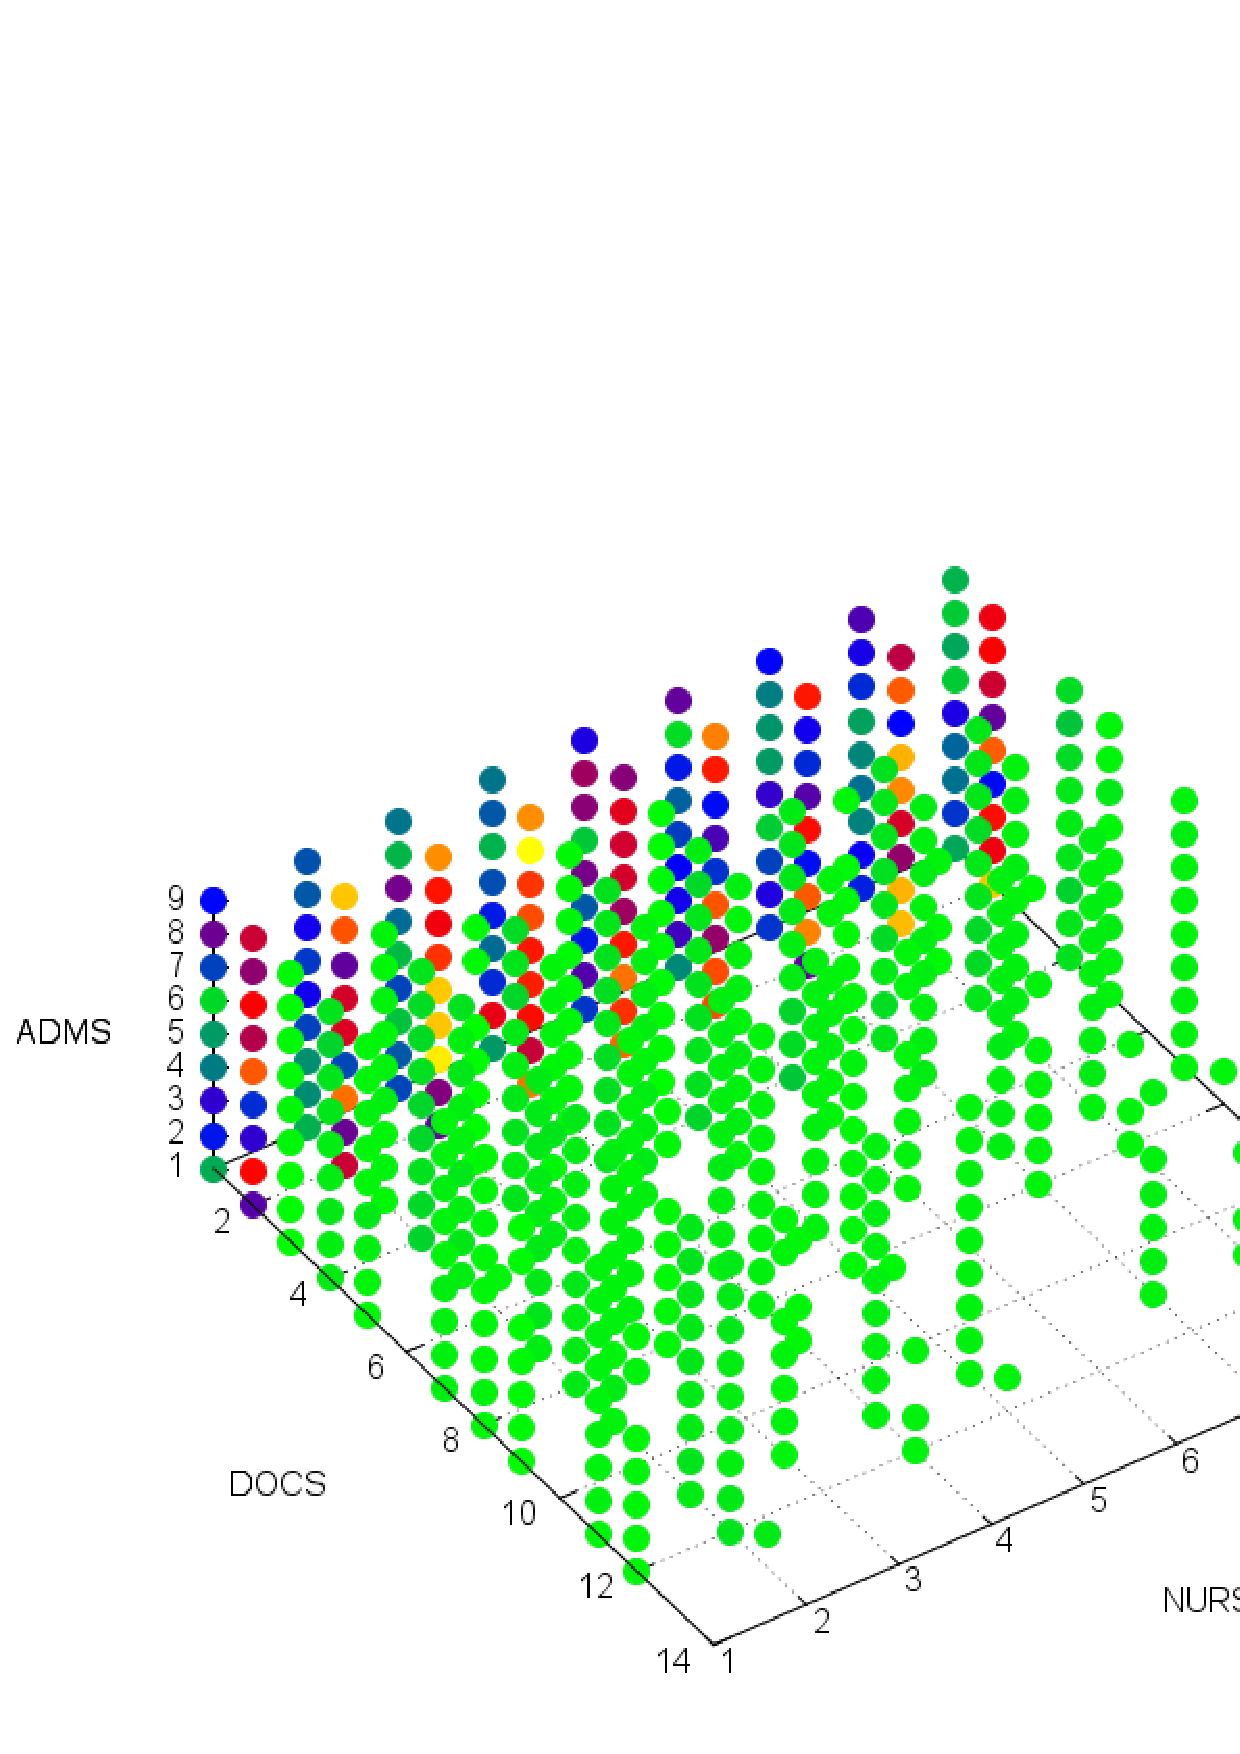
\includegraphics[width=0.88\columnwidth,height=0.2\paperheight]{figs4/3D-scatter-LoS-wo2}\caption{3D scattered graph ordered by the sort and number of staff \ref{subtab:As}
to \ref{subtab:Ds}. The green values of interest were totally scattered.
\label{fig:3D-scattered-LoS-wo}}
\end{figure}
 The second example, \ref{fig:3D-scattered-LoS-cost} shows the index
value ordered by the cost of the sanitary staff configuration. The
green points were less scattered, but blue values and others were
mixed, showing a region not totally connected. Finally, the third
example, \ref{fig:3D-scattered-LoS-tpipe}, shows the index value
ordered by the equivalent operational patient-service time \foreignlanguage{american}{(t{*})}
of each sanitary staff configuration of \ref{subtab:As-pipe} to \ref{subtab:XRs-pipe}.
This graph shows a connected and almost ``non'' scattered green
region. %
\begin{comment}
As a result of using this equivalent operational patient-service time
\foreignlanguage{american}{(t{*})} order of each staff configuration
the axes were unique and in ascending order. 
\end{comment}


\begin{figure}[h]
\noindent \begin{centering}
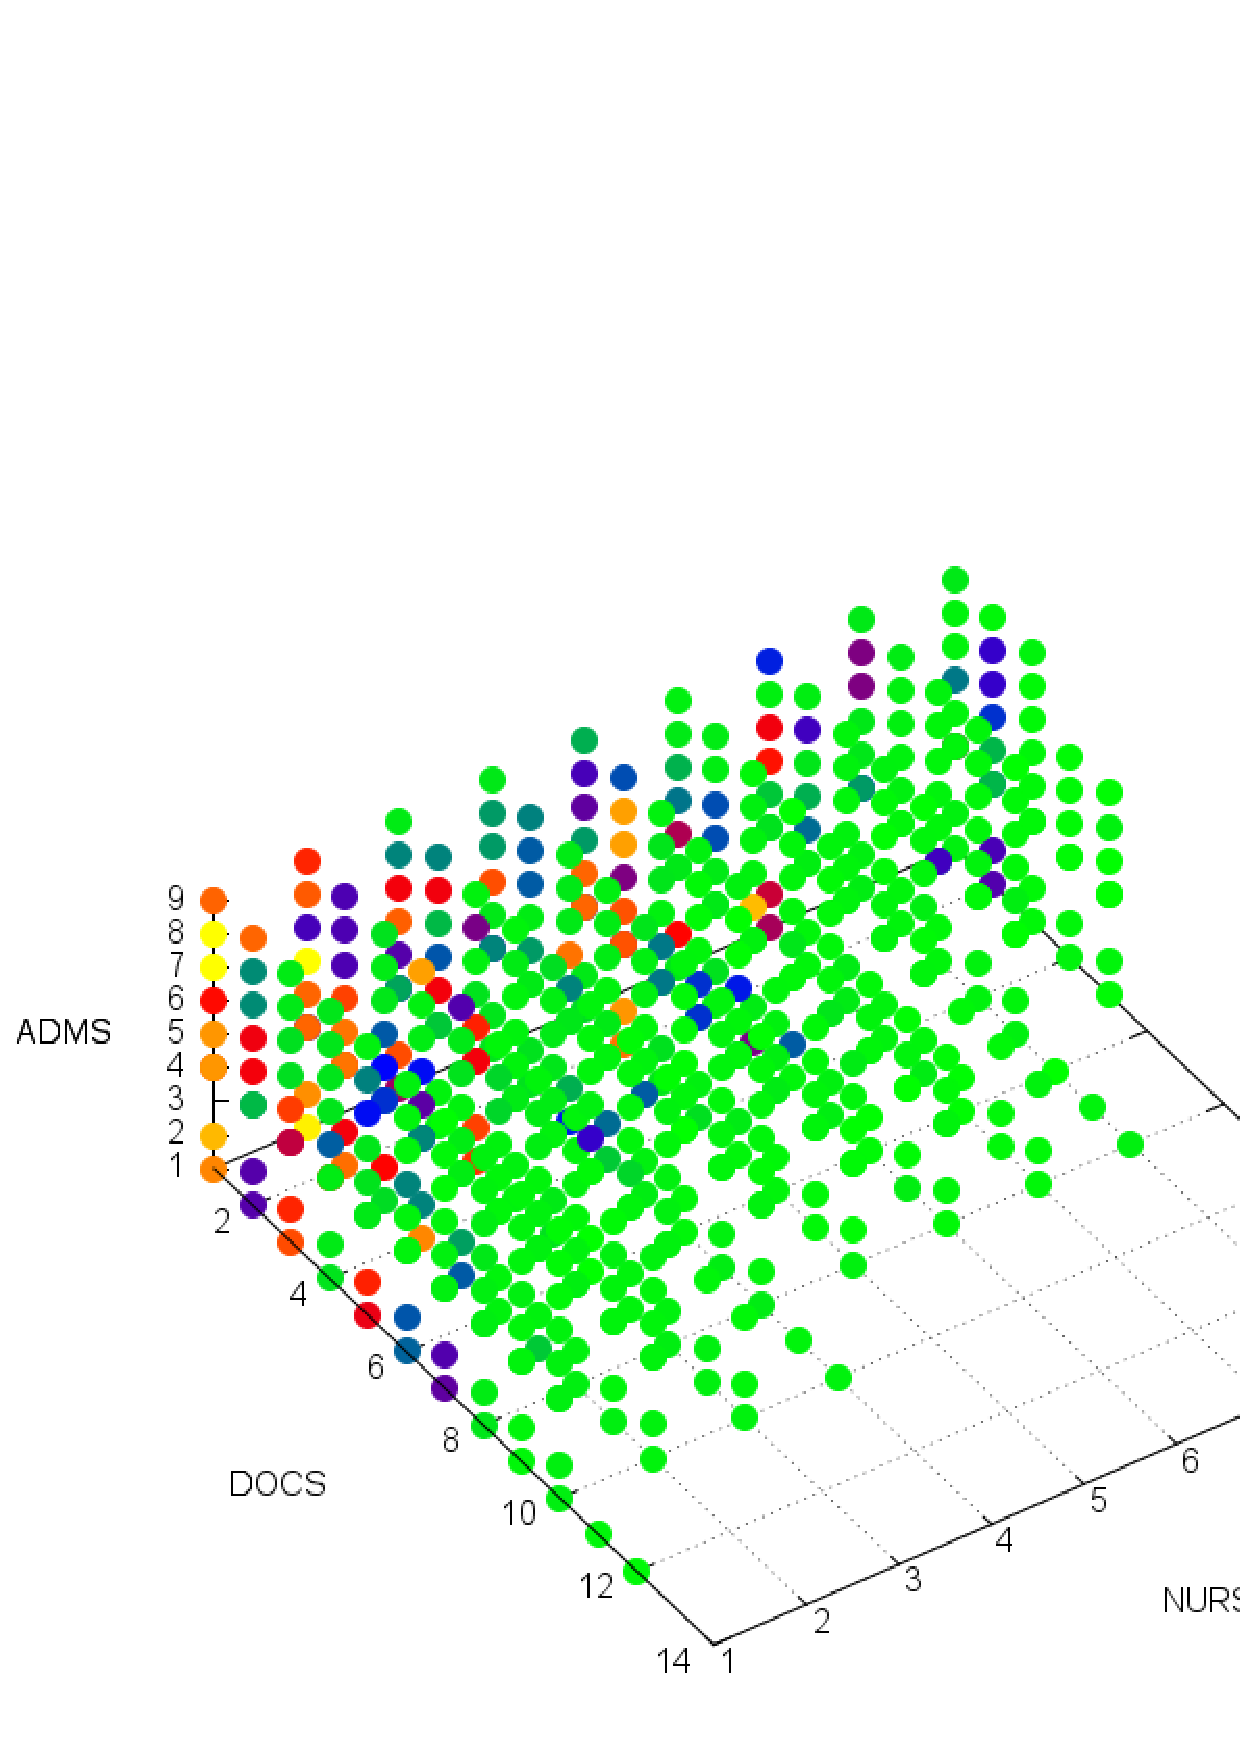
\includegraphics[width=0.88\columnwidth,height=0.2\paperheight]{figs4/3D-scatter-LoS-$2}
\par\end{centering}

\caption{3D scattered graph ordered by the cost of sanitary staff configuration.
The green values of interest were not so scattered, but not interconnected.\label{fig:3D-scattered-LoS-cost} }


\end{figure}


\section{Workloads}

In order to analyse the performance of the ED, the real average four
hundred incoming patients daily arrive to the ED of Sabadell hospital
was considered as follows. This real input was divided into four scenarios,
i.e., four different workload scenarios, up to: 4, 9, 13, and 17 incoming
patients hourly, as shown in \ref{tab:scenarios} (i.e., up to 96,
216, 312, and 408, respectively for 24hrs.).
\begin{figure}[H]
 %
\noindent \begin{centering}
\centering\foreignlanguage{british}{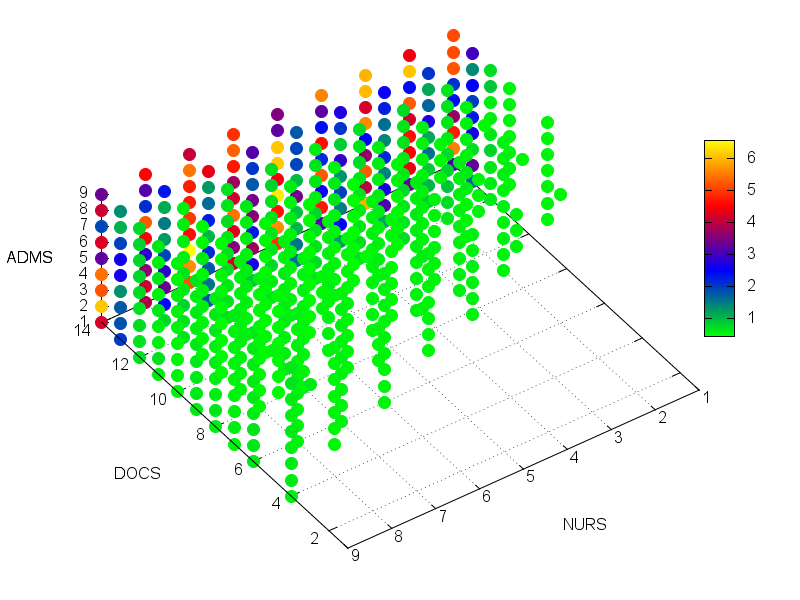
\includegraphics[width=0.88\columnwidth,height=0.2\paperheight]{figs4/3D-scatter-LoS-tpipe2}}
\par\end{centering}

  %
\caption{3D scattered graph ordered by the equivalent operational patient-service
time \foreignlanguage{american}{(t{*})} of a ``single one'' sanitary
professional of each sanitary staff configuration \ref{subtab:As-pipe}
to \ref{subtab:XRs-pipe}. The green value region of interest was
connected and almost ``non'' scattered.\label{fig:3D-scattered-LoS-tpipe} }
\end{figure}
 These different workload scenarios were used to supply different
loads to the ED, whereas the percentage of the priority level of patients
was maintained. 

\begin{table}[H]
\centering{}\caption{Incoming ED patients divided into four different workload scenarios,
up to: 4, 9, 13, and 17 patients per hour for each scenario. \label{tab:scenarios}}
\resizebox{2.3in}{!}{ %
\begin{tabular}{>{\centering}m{3.7cm}>{\centering}m{3.75cm}}
\hline 
Workload scenario number & \textbf{Incoming patients (hourly)} \tabularnewline
\hline 
1 & 4\tabularnewline
2 & 9\tabularnewline
3 & 13\tabularnewline
4 & 17\tabularnewline
\hline 
\end{tabular}}
\end{table}
\clearpage{}


\section{Evaluation Metrics}

The set of metrics used in this work were: the length of stay (LoS)
of the patients in the ED; the number of attended patients per day
(Throughput); and a compound index, the product of the cost of a given
sanitary staff configuration times patient length of stay (CLoS).

Furthermore, the computing time of each of the proposed optimisation
method is measured in order to observe the gains in reducing computing
time of the methodology proposed.\\


All simulations of the ED optimization cases analysed in this work
were carried out in a Linux cluster of the CAOS Department of the
UAB, which has 608 computing cores and 2.2TB of RAM, that is composed
of: 9 nodes of a dual-4 core Intel Xeon E5430, 2.6GHz, 16GB RAM; 1
node of 2xdual-6 core Intel Xeon E5645, 2.4GHz, 24GB RAM; and 8 nodes
of 4x16-cores AMD Opteron ``Interlagos'', 1.66GHz, 256 GB RAM, all
in a switched 1GigE network.


\section{Evaluation Method}

The evaluation of the proposed methodology was aimed to confirm the
correct operation of both the pipeline approach (PA) and the MC plus
the K-means methods, described in \ref{chap3:Math}. To this end,
we have first performed the exhaustive search (ES) to use as baseline
method. The second step of this evaluation consists on applying the
coarse grained phase, using either the PA, the MC plus K-means methods,
or both. Finally, the fine grained phase is apply in the promising
regions found in the previous step. 

In order to evaluate quantitatively the proposal methodology two case
studies were set. The first of them, namely case study A, was performed
using the agent-based ED simulator version 1.1. This case study is
further described in \ref{sub:Case-Study-A}. The second case or case
study B was performed using the agent-based ED simulator version 1.2
(the current version). This case study is further described in \ref{sub:Case-Study-B}.

In both case studies, only patients identified as triage level 4 and
5 are served at the stage of diagnosis-treatment phase, the three
metrics, and the four different workloads stated above were tested,
and the period simulated was 24 hrs., i.e., one day of functioning
of the ED, in all the experiments. Test scenarios and evaluation results
of both case studies are explained in detail in the following sections.\\


It is important to remind that the actions and interactions corresponding
to the admission and triage processes have been totally implemented,
but in the case of diagnostic and treatment phase, respecting to the
priorities of the Sabadell Hospital ED currently only the level 1
was implemented. In such level 1 only patients identified with priority
level 4 or 5 (less urgent, and non-urgent, respectively \ref{sec:active-agents})
were taken care of. Nevertheless, all incoming patients were triaged.
Once patients have been triaged, only patients identified as triage
level 4 and 5 were served at the stage of diagnosis-treatment phase.


\section{Case Study B \label{sub:Case-Study-B}}

The agent-based ED simulator v1.2, which is shown in \ref{fig:ED-SIM-2-1},
was used in this case study. 
\begin{figure}[h]
\noindent \begin{centering}
\includegraphics[width=0.95\columnwidth,height=0.21\paperheight]{figs4/ED-v1\lyxdot 0}
\par\end{centering}

\caption{ED simulator v1.2. Admission personnel, triage nurses, doctors, emergency
nurses, and x-ray technicians were the sanitary staff considered.\label{fig:ED-SIM-2-1}}
\end{figure}
 In this version of the ED simulator the diagnosis and treatment phase
is more detailed, because the diagnosis tests were done by other agents,
x-ray technicians or emergency nurses, or both. The simple patient
flow in the such current v1.2 of the ED simulator is defined as follows:
patients arrive to the ED on their own, and waits to be attended in
the admission area. Then, patients stay in the first Waiting Room
(WR) WR1, until a triage nurse call them. After the triage process
patients identified as triage level 4 and triage level 5 pass to a
second WR2, and stay there until a free doctor calls them to begin
the diagnosis-treatment phase (interrogation process), depending on
the patient's symptoms and physical condition, patients wait at WR
(Level 1) to be attended by an x-ray technician or an emergency nurse
(to perform some diagnostic tests). After tests, patients come back
to WR (Level 1) and stay there until a free doctor calls them again
(treatment process). At the end, patients are discharged from the
ED. 

It was found through interviews with the managers at the ED of Sabadell
that the 100\% of patients undergo interrogation phase; the 80\% of
patients required to perform some diagnostic tests; and only 20\%
need to apply a treatment. These percentages are common for patients
identified as triage level 4 and 5.

Therefore, in this case study the sanitary staff considered were:
admission personnel, triage nurses, emergency nurses, doctors, and
x-ray technicians. It is a 5D problem. Thus, the \ref{subtab:As-pipe}
to \ref{subtab:XRs-pipe} were taken into account. As a result, 28,350
($14D*9N*9A*5En*5Xr$) staff configurations were tested for each of
the four workload scenarios of incoming patients stated in \ref{tab:scenarios}. 

Finally, the three metrics above stated: LoS, Throughput, and CLoS
were performed using two methods: the exhaustive search technique
(ES), and the coarse grained phase, using only the MC plus K-means
methods. Finally, the fine grained phase was applied in the reduced
feasible region to find the optimum.


\subsection{LoS Index}

This objective set was to minimise patient length of stay (LoS), with
cost constraint less or equal to 5,500�. It is expressed mathematically
in \ref{eq:LoS index-2}:

\begin{equation}
\begin{aligned} & {\text{Minimise LoS}} &  & f(D,N,A,En,Xr)\\
 & \text{subject to} &  & D_{cost}+N_{cost}+A_{cost}+En_{cost}+\\
 &  &  & Xr_{cost}\in Cost\leq5,500\:\text{�}
\end{aligned}
\label{eq:LoS index-2}
\end{equation}


It is worth noting that each of the plotted points for the following
four workload scenarios were obtained running the ED simulator as
many times as points are, that correspond to each of the 23,445 staff
configurations (out of 28,350) that satisfy the cost restriction.

\clearpage{}


\subsubsection{First Workload Scenario}

The results of this scenario, up to 4 patients/hour, are shown from
\ref{subfig:es4-4} to \ref{subfig:km4-4}. The ES result is shown
in \ref{subfig:es4-4}, where the red triangle was the minimum. 
\begin{figure}[H]
\centering{}\includegraphics[width=1\columnwidth,height=0.2\paperheight]{figs4/v1\lyxdot 1/v1-25-exh-LoS-min}\caption{Average LoS obtained by the ES method. The red triangle was the minimum.\label{subfig:es4-4}}
\end{figure}


The MC plus the K-means methods results are shown in \ref{subfig:mc4-4}
to \ref{subfig:km4-4}, respectively. The MC method found 600 configurations.
\begin{figure}[H]
\centering{}\includegraphics[width=1\columnwidth,height=0.2\paperheight]{figs4/v1\lyxdot 1/MC-518400-23445-25-69-25-600confs-LoS}\caption{Average LoS of 600 configurations obtained by the MC method.\label{subfig:mc4-4}}
\end{figure}
 However, it was difficult to get any conclusion about such region;
therefore, the complementary K-means method was performed. The K-means
method identified two different clusters, shown in \ref{subfig:km4-4},
the most important was the green cluster, which delimited the region
where the optimum was.

\begin{comment}
The graphics \ref{subfloat:pipe4} and \ref{subfloat:contour4} shown
another way to visualise the connectivity characteristic of the reduced
regions found by the AP, and the MC plus the K-means methods. In such
connected reduced regions the ``reduced exhaustive search'' is applied.
The axes of such graphs are the first column of \ref{subtab:As-pipe},
\ref{subtab:Ns-pipe}, and \ref{subtab:Ds-pipe}, where they were
ordered by the pipeline approach (PA) \ref{eq:Pipeline formula}.
\end{comment}
\begin{comment}
\begin{figure}[H]
\noindent \begin{centering}
\begin{minipage}[t]{0.45\linewidth}%
\noindent \begin{center}
\includegraphics[width=1\columnwidth]{figs4/v1.1/v1-25-exh-LoS-min.png}
\par\end{center}

\noindent \begin{center}
\caption{}

\par\end{center}%
\end{minipage}
\par\end{centering}

\noindent \begin{centering}
\vfill{}

\par\end{centering}

\begin{minipage}[t]{0.45\textwidth}%
\noindent \begin{center}
\includegraphics[width=1\columnwidth]{figs4/v1.1/MC-518400-23445-25-69-25-600confs-LoS.png}
\par\end{center}

\caption{}
%
\end{minipage}\hfill{}%
\begin{minipage}[t]{0.45\textwidth}%
\noindent \begin{center}
\includegraphics[width=1\columnwidth]{figs4/v1.1/K-means-518400-23445-25-69-25-600-Cluster1-107_Cluster2-486.png}
\par\end{center}

\caption{}
%
\end{minipage}
\end{figure}
\end{comment}


Finally, after applied the MC plus the K-means methods, the \textquotedblleft{}reduced
exhaustive search\textquotedblright{} was performed in such reduced
region identified. The optimum found per each method: the ES, and
the MC plus the K-means methods are presented in \ref{tab:4p-d},
where the sanitary staff configuration (doctors, triage nurses, emergency
nurses, x-ray technicians, and admission personnel), their associated
average minimum LoS, and cost configuration are shown. The two optima
independently found were the same. 
\begin{figure}[H]
\begin{centering}
\includegraphics[width=1\columnwidth,height=0.2\paperheight]{figs4/v1\lyxdot 1/K-means-518400-23445-25-69-25-600-Cluster1-107_Cluster2-486}
\par\end{centering}

\caption{The K-means method identified two clusters of average LoS. The green
one delimited the region where the minimum was.. \label{subfig:km4-4}}
\end{figure}


\begin{table}[H]
\caption{Optimum staff configurations that got the average minimum LoS for
this workload scenario (up to 4 patients hourly), where S is Senior
and J is Junior. It is shown in red triangle in \ref{subfig:es4-4}.}


\begin{centering}
\begin{tabular}{cc>{\centering}p{1.3cm}ccccc>{\centering}p{2.8cm}}
\hline 
Method & � & LoS (hrs) & D & N & A & EN & XR & Run time (hrs)

256 Pthreads)\tabularnewline
\hline 
ES & 3,850 & 3.7 & 1S,3J & 1J & 1J & 1S & 1S,1J & 2.5\tabularnewline
MC+K-means & 3,850 & 3.7 & 1S,3J  & 1J & 1J  & 1S & 1S,1J & 0.84\tabularnewline
\hline 
\end{tabular}
\par\end{centering}

\label{tab:4p-d} 
\end{table}



\subsubsection{Second Workload Scenario}

The results of this scenario, up to 9 patients/hour, are shown from
\ref{subfig:es8-4} to \ref{subfig:km8-4}. The ES result is shown
in \ref{subfig:es8-4}, where the red triangle was the minimum. 

The MC plus the K-means methods results are shown in \ref{subfig:mc8-4}
to \ref{subfig:km8-4}, respectively. The MC method found 150 configurations.
However, it was difficult to get any conclusion about such region;
therefore, the complementary K-means method was performed. The K-means
method identified two different clusters, shown in \ref{subfig:km8-4},
the most important was the red cluster, which delimited the region
where the optimum was.

\begin{comment}
The graphics \ref{subfloat:pipe4} and \ref{subfloat:contour4} shown
another way to visualise the connectivity characteristic of the reduced
regions found by the AP, and the MC plus the K-means methods. In such
connected reduced regions the ``reduced exhaustive search'' is applied.
The axes of such graphs are the first column of \ref{subtab:As-pipe},
\ref{subtab:Ns-pipe}, and \ref{subtab:Ds-pipe}, where they were
ordered by the pipeline approach (PA) \ref{eq:Pipeline formula}.
\end{comment}
\begin{comment}
\begin{figure}[H]
\noindent \begin{centering}
\begin{minipage}[t]{0.45\linewidth}%
\noindent \begin{center}
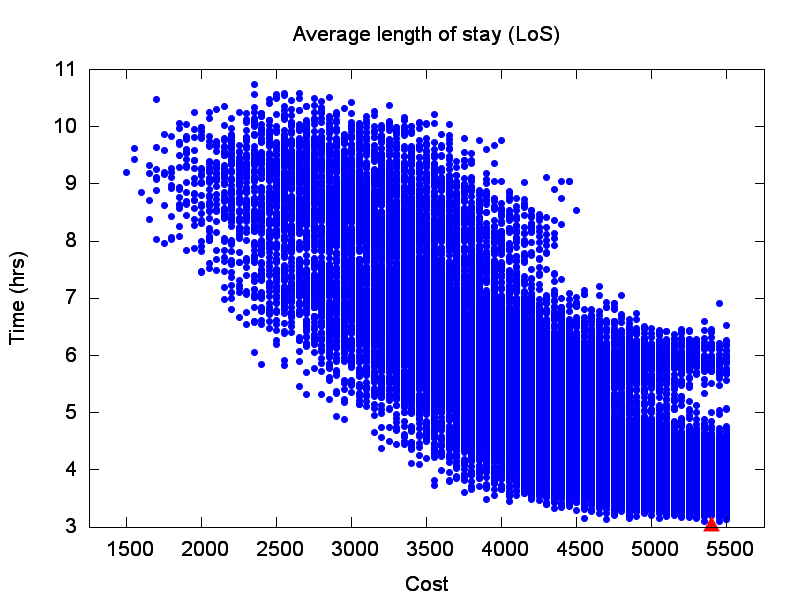
\includegraphics[width=1\columnwidth]{figs4/v1.1/v1-50-exh-LoS-min.png}
\par\end{center}

\noindent \begin{center}
\caption{Average LoS obtained by the ES method. The red triangle was the minimum. }

\par\end{center}%
\end{minipage}
\par\end{centering}

\noindent \begin{centering}
\vfill{}

\par\end{centering}

\begin{minipage}[t]{0.45\textwidth}%
\noindent \begin{center}
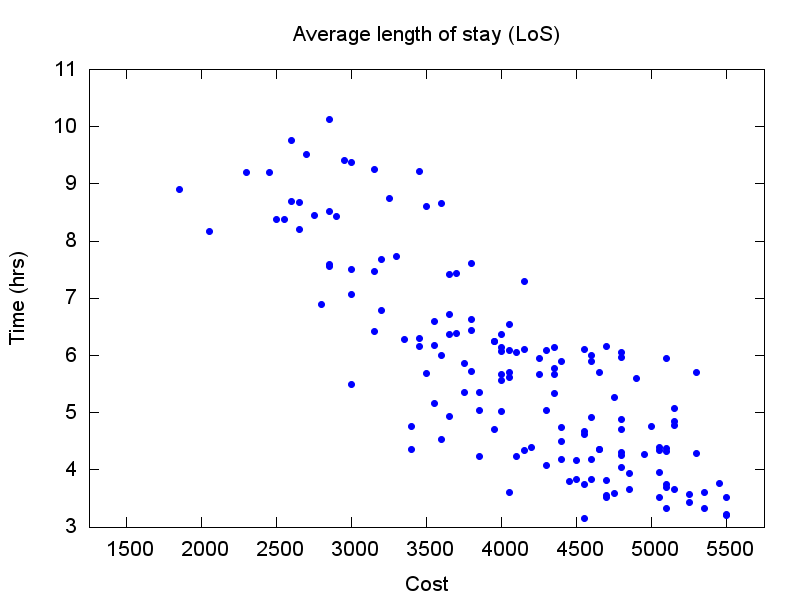
\includegraphics[width=1\columnwidth]{figs4/v1.1/MC-518400-23445-50-69-25-150confs-LoS.png}
\par\end{center}

\caption{Average LoS of 150 configurations obtained by the MC method.}
%
\end{minipage}\hfill{}%
\begin{minipage}[t]{0.45\textwidth}%
\noindent \begin{center}
\includegraphics[width=1\columnwidth]{figs4/v1.1/K-means-518400-23445-50-69-25-150-Cluster1-105_Cluster2-45.png}
\par\end{center}

\caption{The K-means method identified two clusters of average LoS. The red
one delimited the region where the minimum was.}
%
\end{minipage}
\end{figure}
\end{comment}


Finally, after applied the MC plus the K-means methods, the \textquotedblleft{}reduced
exhaustive search\textquotedblright{} was performed in such reduced
region identified. The optimum found per each method: the ES, and
the MC plus the K-means methods are presented in \ref{tab:8p-d},
where the sanitary staff configuration (doctors, triage nurses, emergency
nurses, x-ray technicians, and admission personnel), their associated
average minimum LoS, and cost configuration are shown. The two optima
independently found were the same. 
\begin{figure}[H]
\centering{}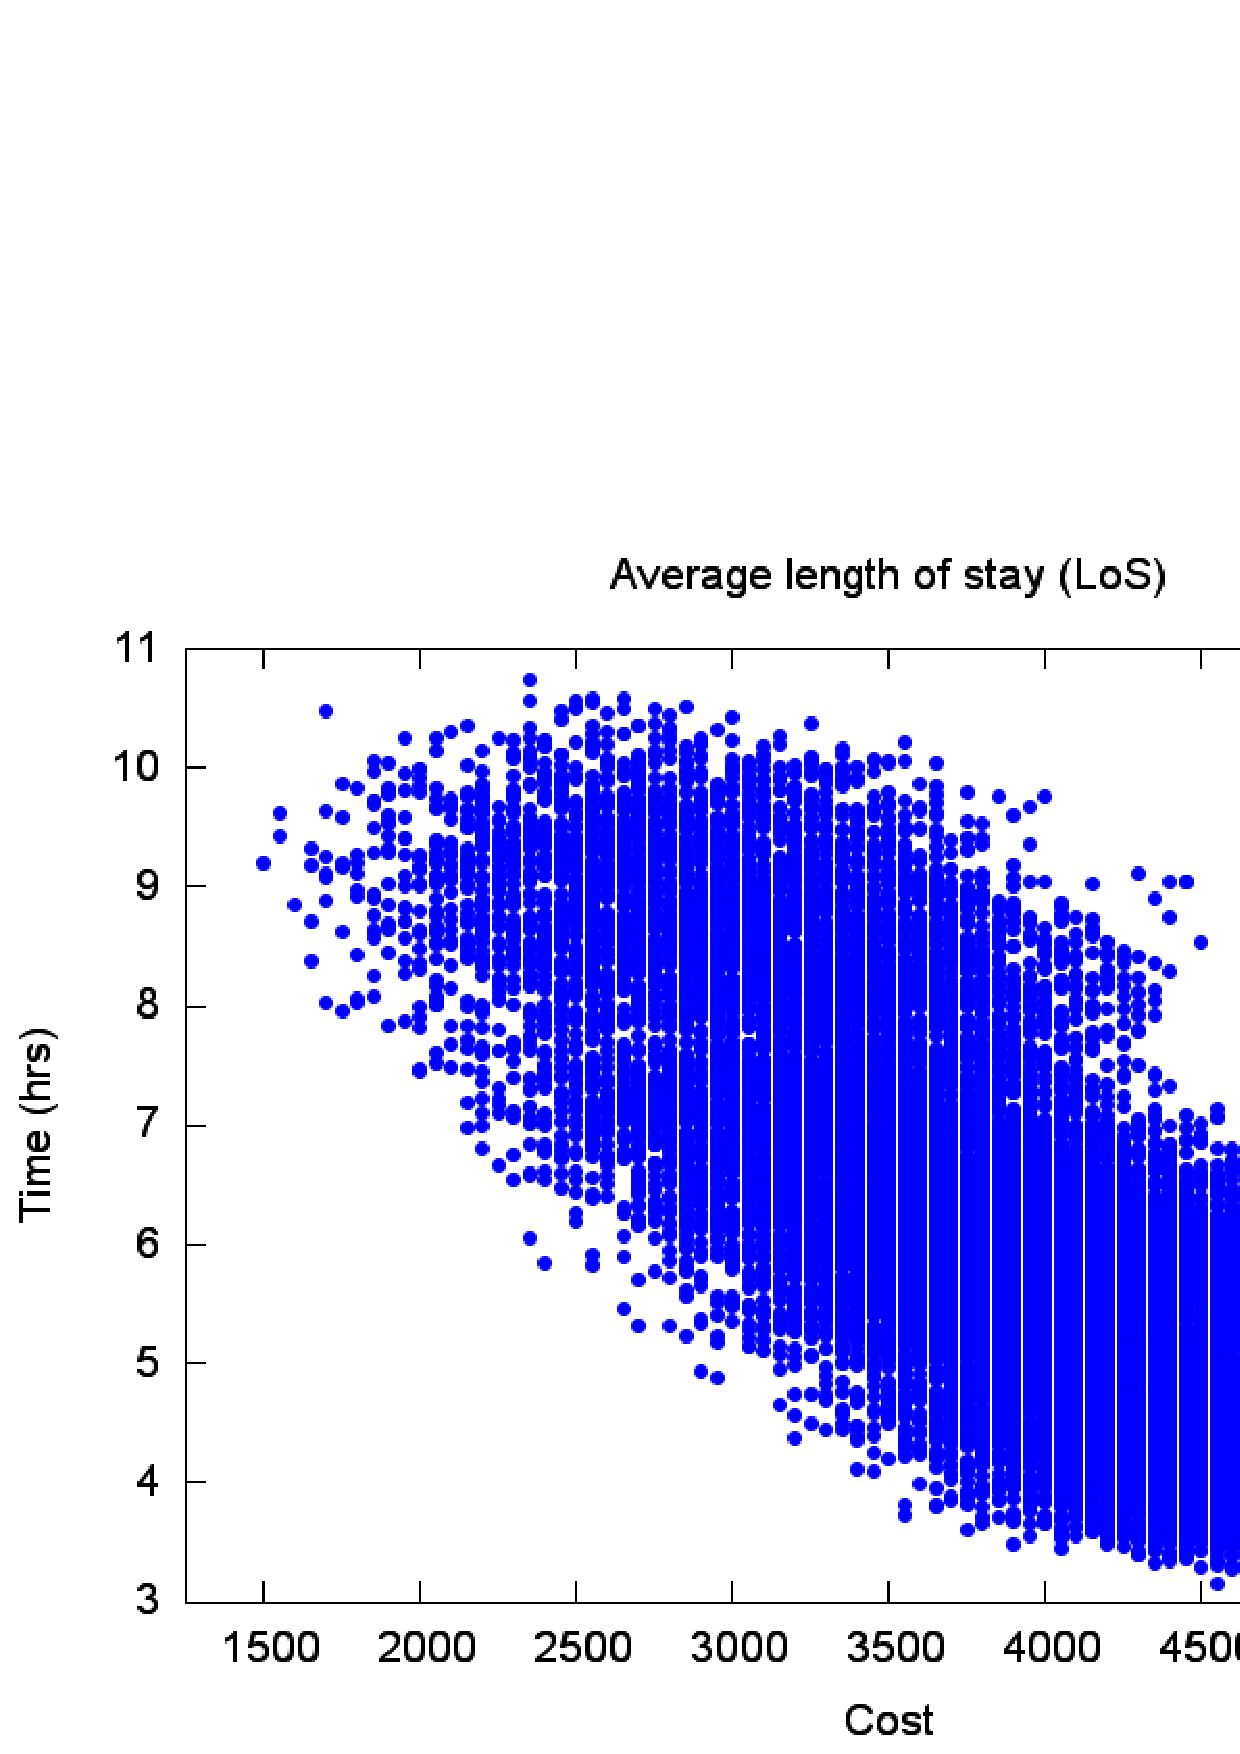
\includegraphics[width=1\columnwidth,height=0.2\paperheight]{figs4/v1\lyxdot 1/v1-50-exh-LoS-min}\caption{Average LoS obtained by the ES method. The red triangle was the minimum.\label{subfig:es8-4}}
\end{figure}
\begin{figure}[H]
\centering{}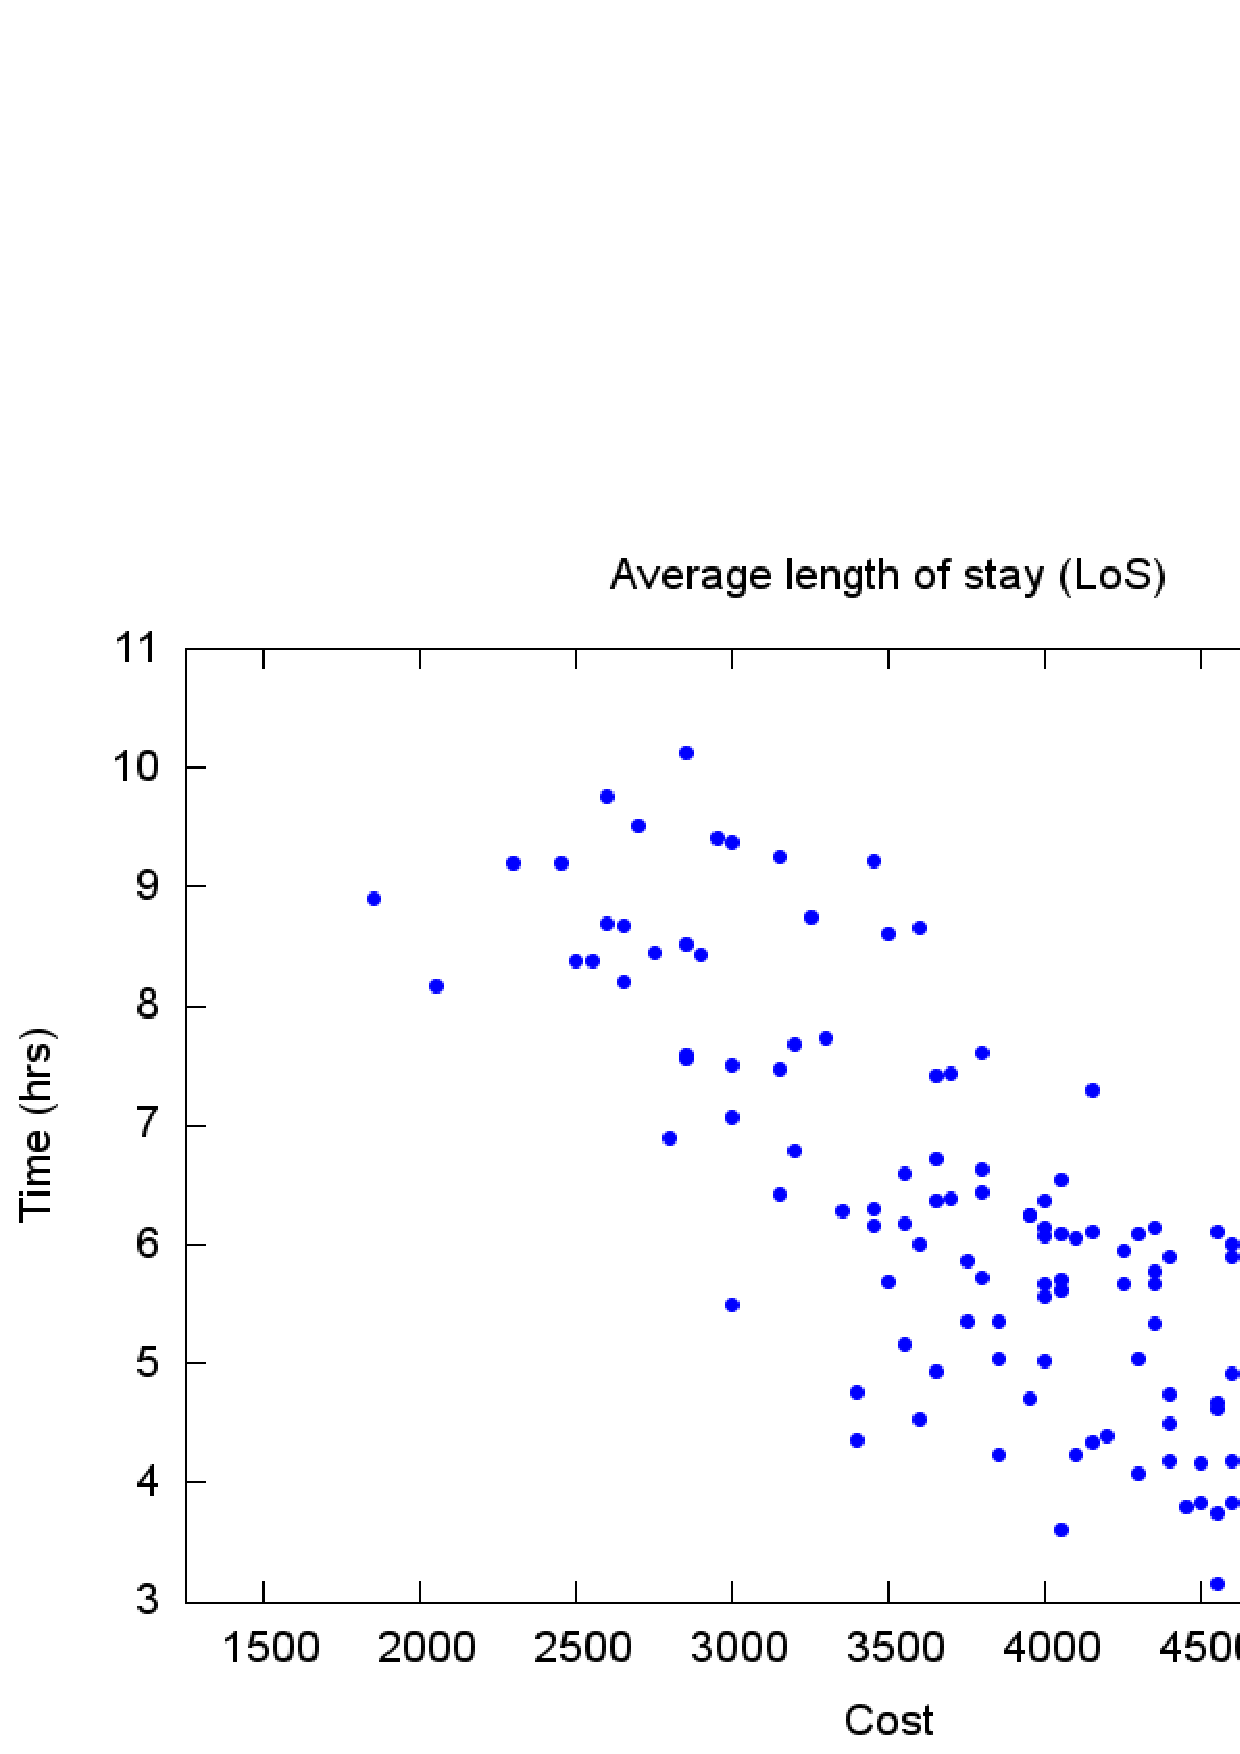
\includegraphics[width=1\columnwidth,height=0.2\paperheight]{figs4/v1\lyxdot 1/MC-518400-23445-50-69-25-150confs-LoS}\caption{Average LoS of 150 configurations obtained by the MC method.\label{subfig:mc8-4}}
\end{figure}


\begin{table}[H]
\caption{Optimum staff configurations that got the average minimum LoS for
this workload scenario (up to 9 patients hourly), where S is Senior
and J is Junior. It is shown in red triangle in \ref{subfig:es8-4}.}


\begin{centering}
\begin{tabular}{cc>{\centering}p{1.3cm}ccccc>{\centering}p{2.8cm}}
\hline 
Method & � & LoS (hrs) & D & N & A & EN & XR & Run time (hrs)

256 Pthreads)\tabularnewline
\hline 
ES & 5,400 & 3.1 & 2S,2J & 3J & 1S,1J & 1J & 2J & 3.07\tabularnewline
MC+K-means & 5,400 & 3.1 & 2S,2J & 3J & 1S,1J & 1J & 2J & 0.57\tabularnewline
\hline 
\end{tabular}
\par\end{centering}

\label{tab:8p-d} 
\end{table}
\begin{figure}[H]
\begin{centering}
\includegraphics[width=1\columnwidth,height=0.2\paperheight]{figs4/v1\lyxdot 1/K-means-518400-23445-50-69-25-150-Cluster1-105_Cluster2-45}
\par\end{centering}

\caption{The K-means method identified two clusters of average LoS. The red
one delimited the region where the minimum was. \label{subfig:km8-4}}
\end{figure}



\subsubsection{Third Workload Scenario}

The results of this scenario, up to 13 patients/hour, are shown from
\ref{subfig:es12-4} to \ref{subfig:km12-4}. The ES result is shown
in \ref{subfig:es12-4}, where the red triangle was the minimum.
\begin{figure}[H]
\centering{}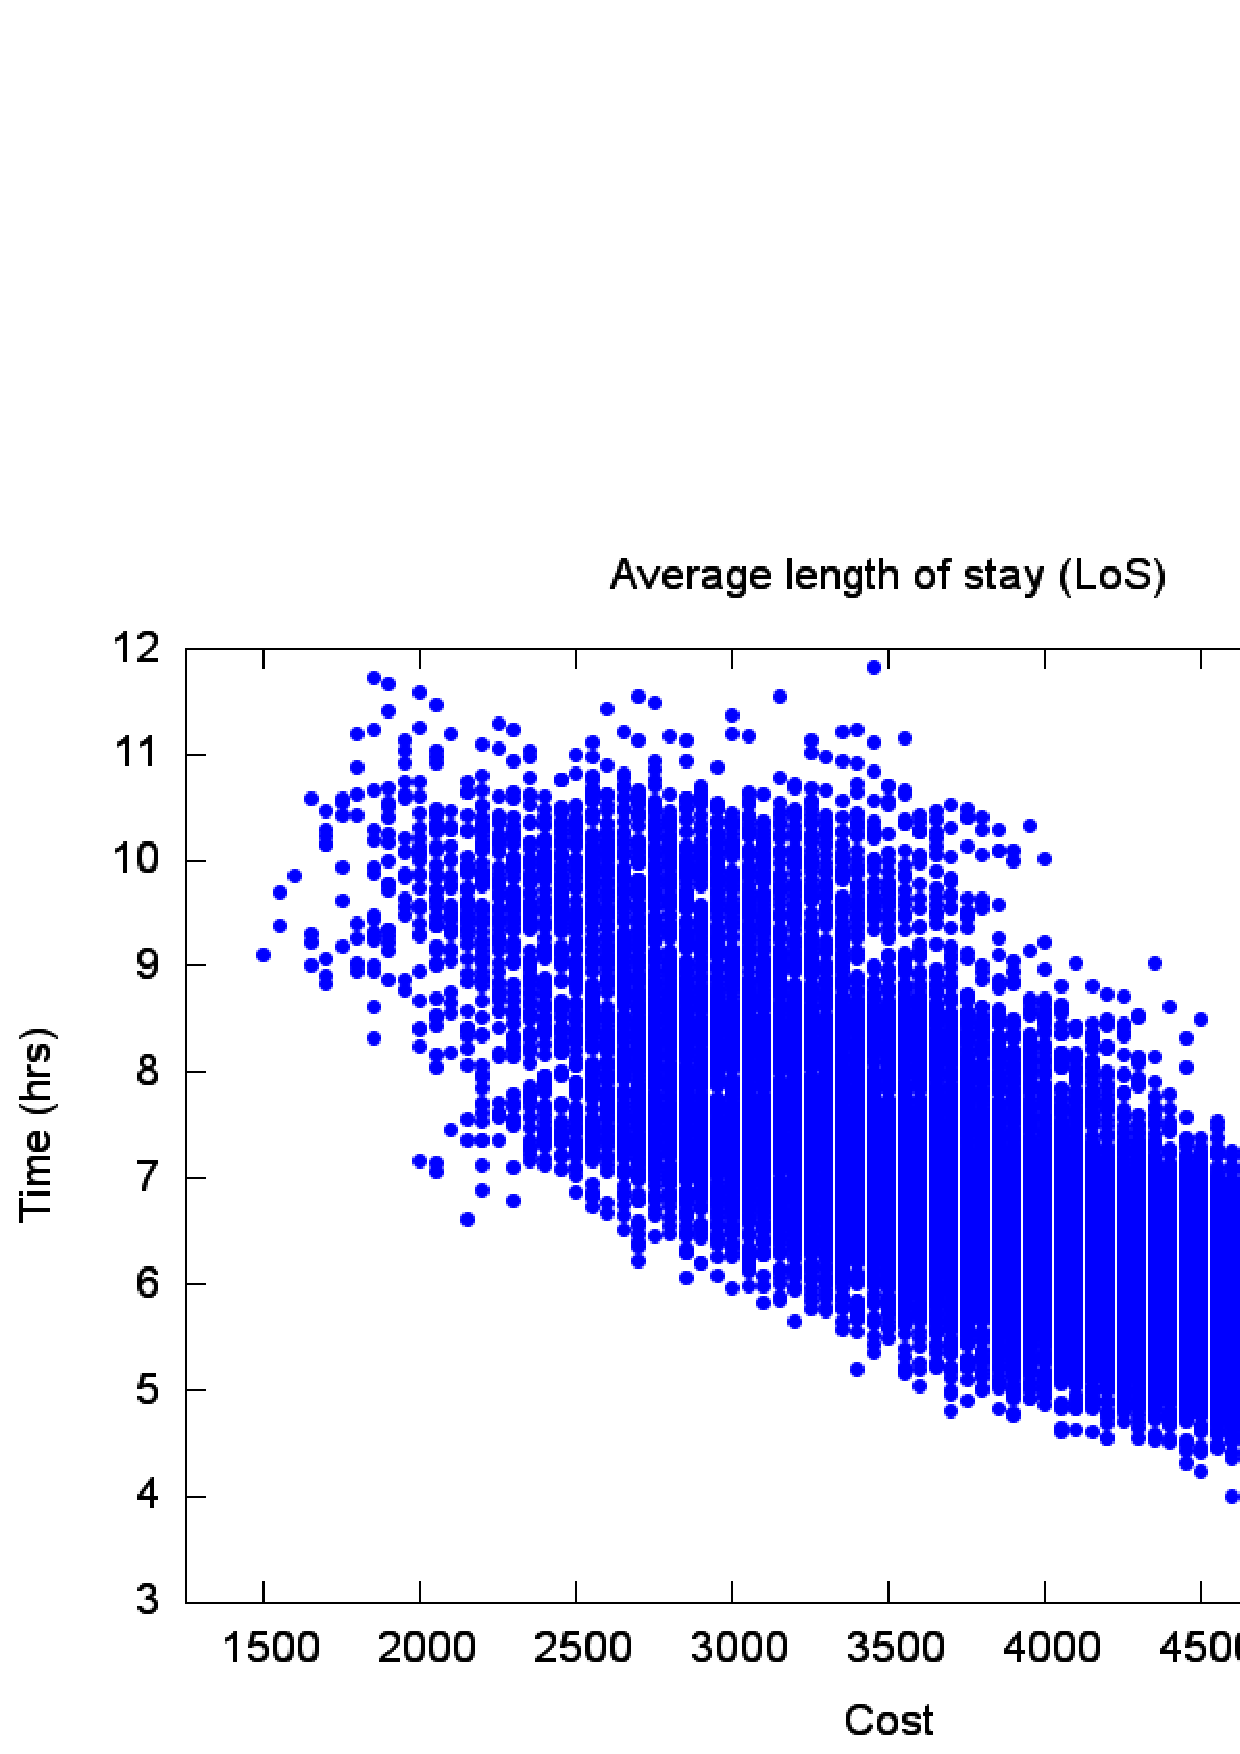
\includegraphics[width=1\columnwidth,height=0.2\paperheight]{figs4/v1\lyxdot 1/v1-75-exh-LoS-min}\caption{Average LoS obtained by the ES method. The red triangle was the minimum.\label{subfig:es12-4}}
\end{figure}


The MC plus the K-means methods results are shown in \ref{subfig:mc12-4}
to \ref{subfig:km12-4}, respectively. The MC method found 150 configurations.
\begin{figure}[H]
\centering{}\includegraphics[width=1\columnwidth,height=0.2\paperheight]{figs4/v1\lyxdot 1/MC-518400-23445-75-69-25-150confs-LoS}\caption{Average LoS of 150 configurations obtained by the MC method.\label{subfig:mc12-4}}
\end{figure}
However, it was difficult to get any conclusion about such region;
therefore, the complementary K-means method was performed. The K-means
method identified two different clusters, shown in \ref{subfig:km12-4},
the most important was the green cluster, which delimited the region
where the optimum was.
\begin{figure}[H]
\begin{centering}
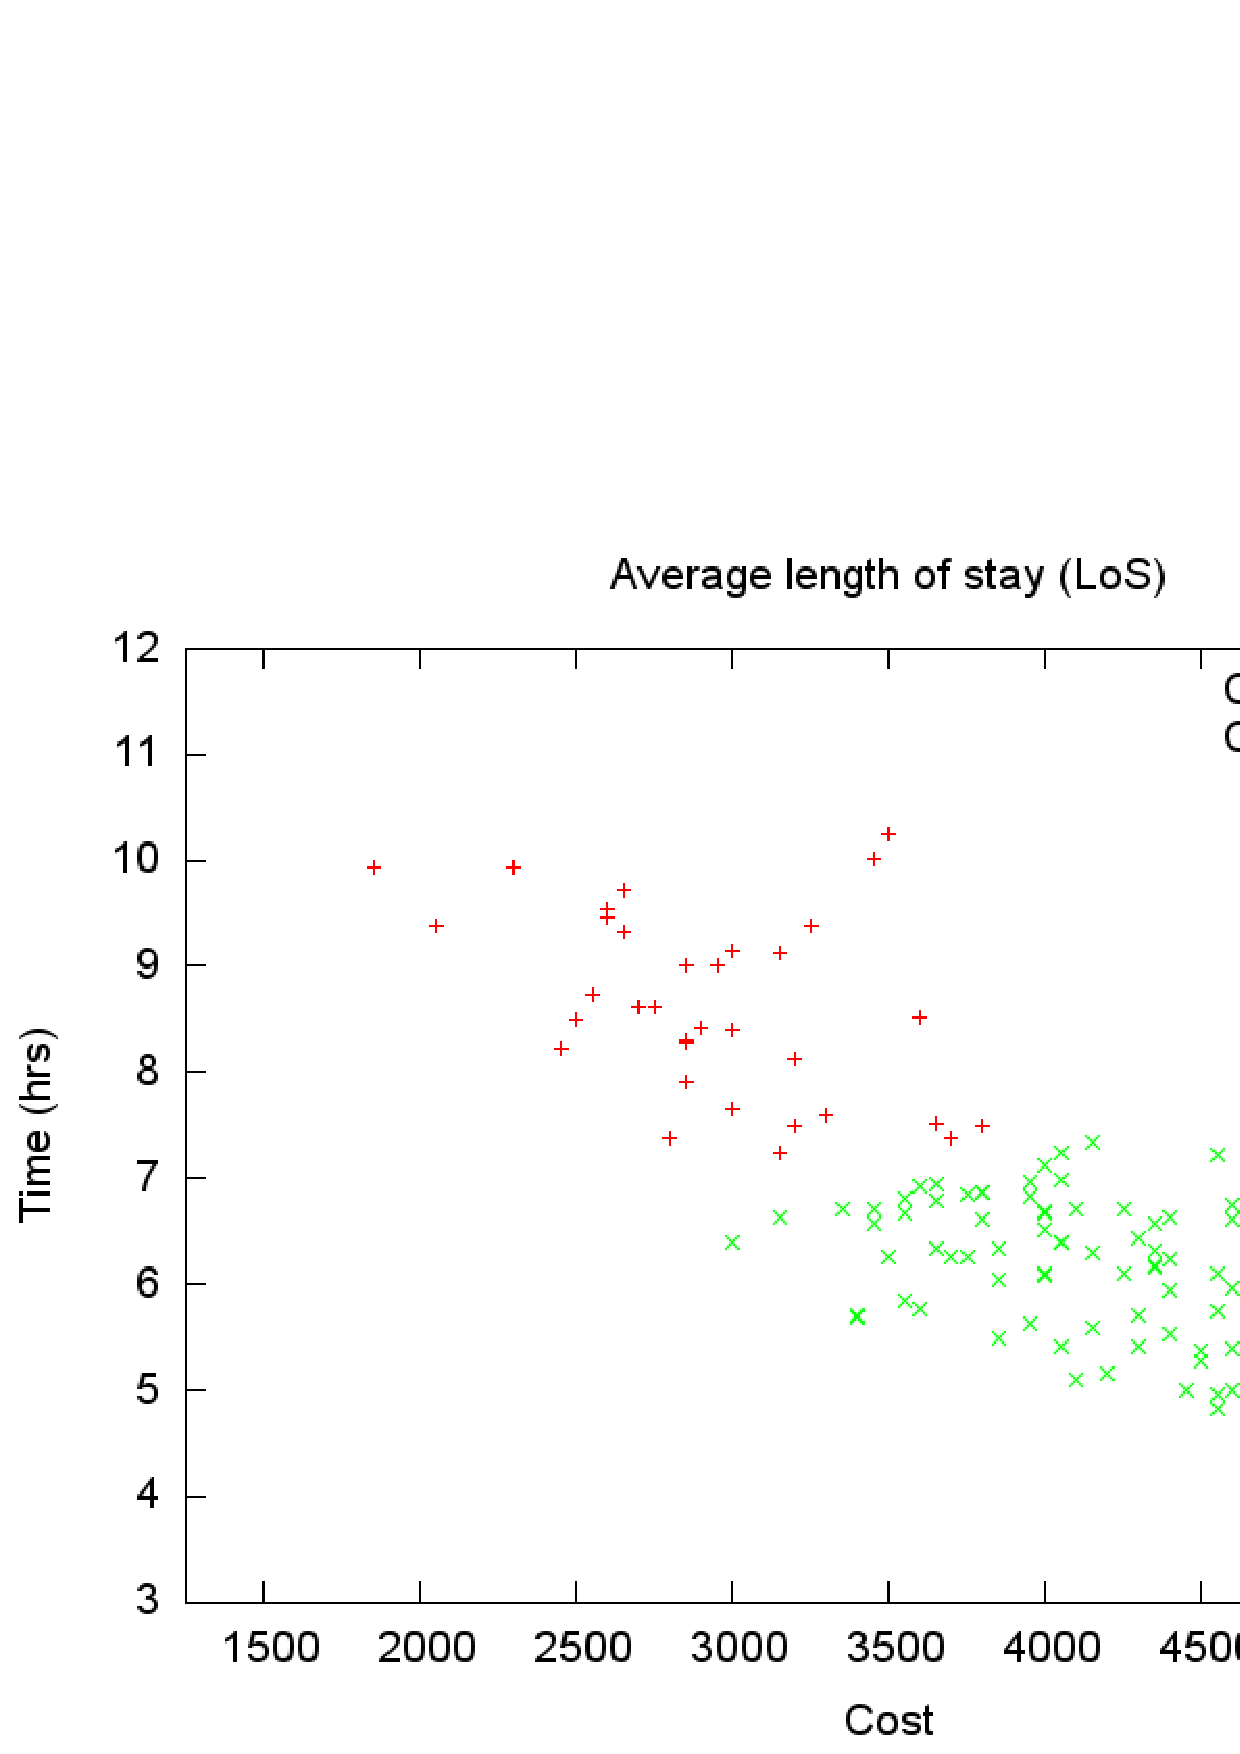
\includegraphics[width=1\columnwidth,height=0.2\paperheight]{figs4/v1\lyxdot 1/K-means-518400-23445-75-69-25-150-Cluster1-34_Cluster2-116}
\par\end{centering}

\caption{The K-means method identified two clusters of average LoS. The green
one delimited the region where the minimum was.\label{subfig:km12-4}}
\end{figure}


\begin{comment}
The graphics \ref{subfloat:pipe4} and \ref{subfloat:contour4} shown
another way to visualise the connectivity characteristic of the reduced
regions found by the AP, and the MC plus the K-means methods. In such
connected reduced regions the ``reduced exhaustive search'' is applied.
The axes of such graphs are the first column of \ref{subtab:As-pipe},
\ref{subtab:Ns-pipe}, and \ref{subtab:Ds-pipe}, where they were
ordered by the pipeline approach (PA) \ref{eq:Pipeline formula}.
\end{comment}
\begin{comment}
\begin{figure}[H]
\noindent \begin{centering}
\begin{minipage}[t]{0.45\linewidth}%
\noindent \begin{center}
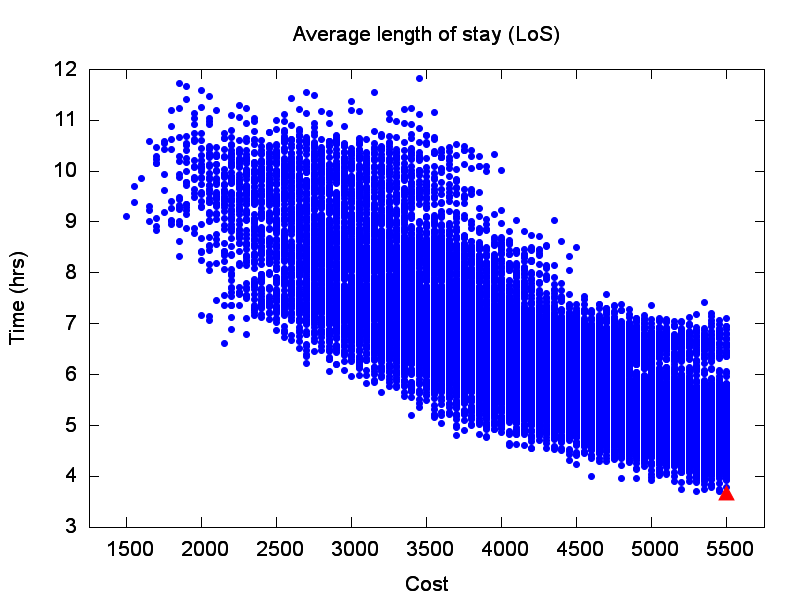
\includegraphics[width=1\textwidth]{figs4/v1.1/v1-75-exh-LoS-min.png}
\par\end{center}

\noindent \begin{center}
\caption{Average LoS obtained by the ES method. The red triangle was the minimum.}

\par\end{center}%
\end{minipage}
\par\end{centering}

\noindent \begin{centering}
\vfill{}

\par\end{centering}

\begin{minipage}[t]{0.45\textwidth}%
\noindent \begin{center}
\includegraphics[width=1\columnwidth]{figs4/v1.1/MC-518400-23445-75-69-25-150confs-LoS.png}
\par\end{center}

\caption{Average LoS of 150 configurations obtained by the MC method.}
%
\end{minipage}\hfill{}%
\begin{minipage}[t]{0.45\textwidth}%
\noindent \begin{center}
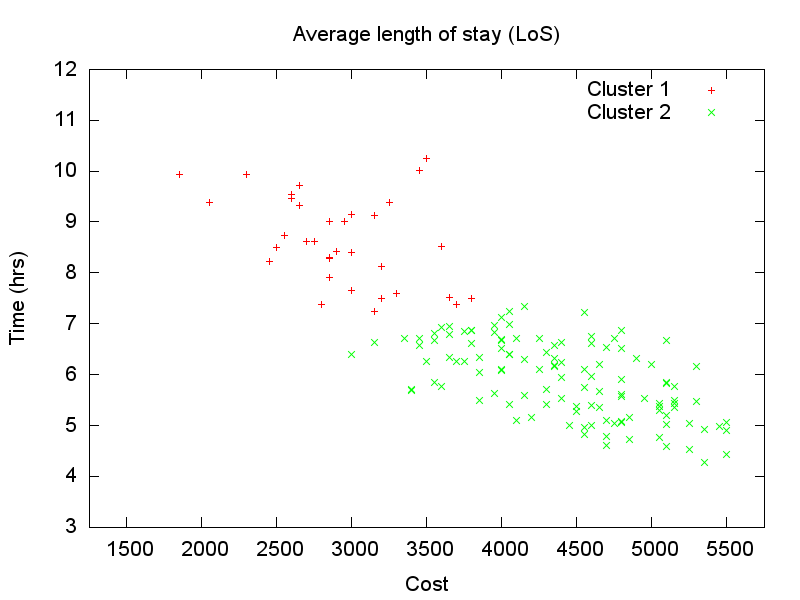
\includegraphics[width=1\columnwidth]{figs4/v1.1/K-means-518400-23445-75-69-25-150-Cluster1-34_Cluster2-116.png}
\par\end{center}

\caption{The K-means method identified two clusters of average LoS. The green
one delimited the region where the minimum was.}
%
\end{minipage}
\end{figure}
\end{comment}


Finally, after applied the MC plus the K-means methods, the \textquotedblleft{}reduced
exhaustive search\textquotedblright{} was performed in such reduced
region identified. The optimum found per each method: the ES, and
the MC plus the K-means methods are presented in \ref{tab:12p-d},
where the sanitary staff configuration (doctors, triage nurses, emergency
nurses, x-ray technicians, and admission personnel), their associated
average minimum LoS, and cost configuration are shown. The two optima
independently found were the same. 

\begin{table}[H]
\caption{Optimum staff configurations that got the average minimum LoS for
this workload scenario (up to 13 patients hourly), where S is Senior
and J is Junior. It is shown in red triangle in \ref{subfig:es12-4}.}


\begin{centering}
\begin{tabular}{cc>{\centering}p{1.3cm}ccccc>{\centering}p{2.8cm}}
\hline 
Method & � & LoS (hrs) & D & N & A & EN & XR & Run time (hrs)

256 Pthreads)\tabularnewline
\hline 
ES & 5,500 & 3.7 & 3S,1J & 2S & 1S,1J & 1J & 2J & 3.72\tabularnewline
MC+K-means & 5,500 & 3.7 & 3S,1J & 2S & 1S,1J & 1J & 2J & 0.56\tabularnewline
\hline 
\end{tabular}
\par\end{centering}

\label{tab:12p-d} 
\end{table}



\subsubsection{Fourth Workload Scenario}

The results of this scenario, up to 17 patients/hour, are shown from
\ref{subfig:es16-4} to \ref{subfig:km16-4}. The ES result is shown
in \ref{subfig:es16-4}, where the red triangle was the minimum.

The MC plus the K-means methods results are shown in \ref{subfig:mc16-4}
to \ref{subfig:km16-4}, respectively. The MC method found 150 configurations.
However, it was difficult to get any conclusion about such region;
therefore, the complementary K-means method was performed. The K-means
method identified two different clusters, shown in \ref{subfig:km16-4},
the most important was the red cluster, which delimited the region
where the optimum was.

\begin{comment}
The graphics \ref{subfloat:pipe4} and \ref{subfloat:contour4} shown
another way to visualise the connectivity characteristic of the reduced
regions found by the AP, and the MC plus the K-means methods. In such
connected reduced regions the ``reduced exhaustive search'' is applied.
The axes of such graphs are the first column of \ref{subtab:As-pipe},
\ref{subtab:Ns-pipe}, and \ref{subtab:Ds-pipe}, where they were
ordered by the pipeline approach (PA) \ref{eq:Pipeline formula}.
\end{comment}
\begin{comment}
\begin{figure}[H]
\noindent \begin{centering}
\begin{minipage}[t]{0.45\linewidth}%
\noindent \begin{center}
\includegraphics[width=1\columnwidth]{figs4/v1.1/v1-100-exh-LoS-min.png}
\par\end{center}

\noindent \begin{center}
\caption{Average LoS obtained by the ES method. The red triangle was the minimum.}

\par\end{center}%
\end{minipage}
\par\end{centering}

\noindent \begin{centering}
\vfill{}

\par\end{centering}

\begin{minipage}[t]{0.45\textwidth}%
\noindent \begin{center}
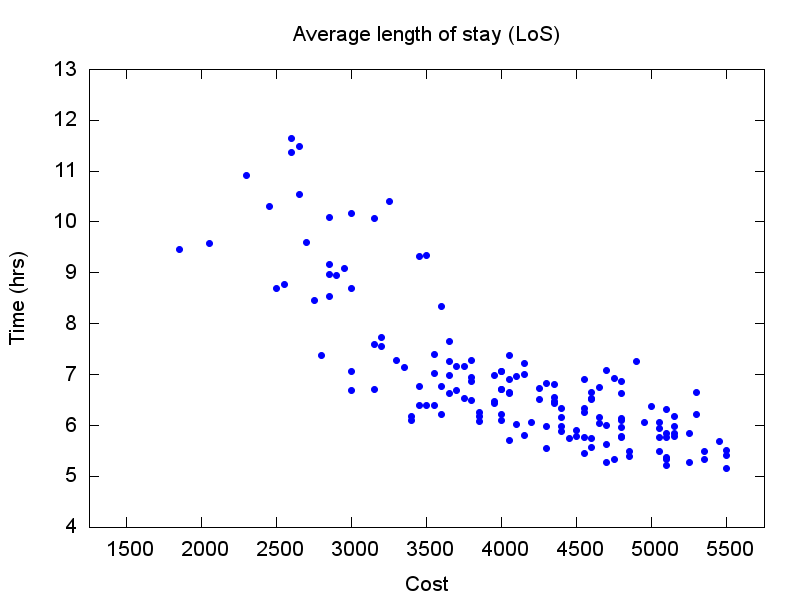
\includegraphics[width=1\columnwidth]{figs4/v1.1/MC-518400-23445-100-69-25-150confs-LoS.png}
\par\end{center}

\caption{Average LoS of 150 configurations obtained by the MC method.}
%
\end{minipage}\hfill{}%
\begin{minipage}[t]{0.45\textwidth}%
\noindent \begin{center}
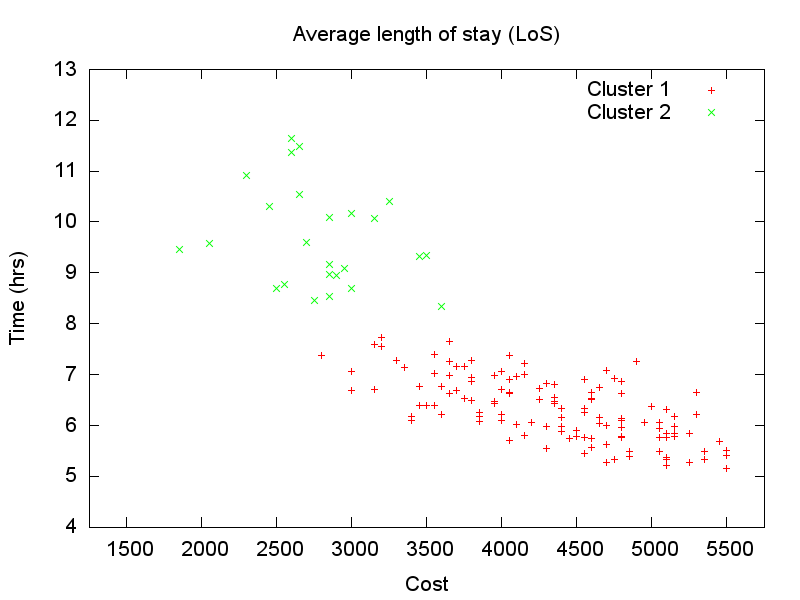
\includegraphics[width=1\columnwidth]{figs4/v1.1/K-means-518400-23445-100-69-25-150-Cluster1-125_Cluster2-25.png}
\par\end{center}

\caption{The K-means method identified two clusters of average number of attended
patients. The red one delimited the region where the minimum was.}
%
\end{minipage}
\end{figure}
\end{comment}
\begin{figure}[H]
\centering{}\includegraphics[width=1\columnwidth,height=0.2\paperheight]{figs4/v1\lyxdot 1/v1-100-exh-LoS-min}\caption{Average LoS obtained by the ES method. The red triangle was the minimum.\label{subfig:es16-4}}
\end{figure}
\begin{figure}[H]
\centering{}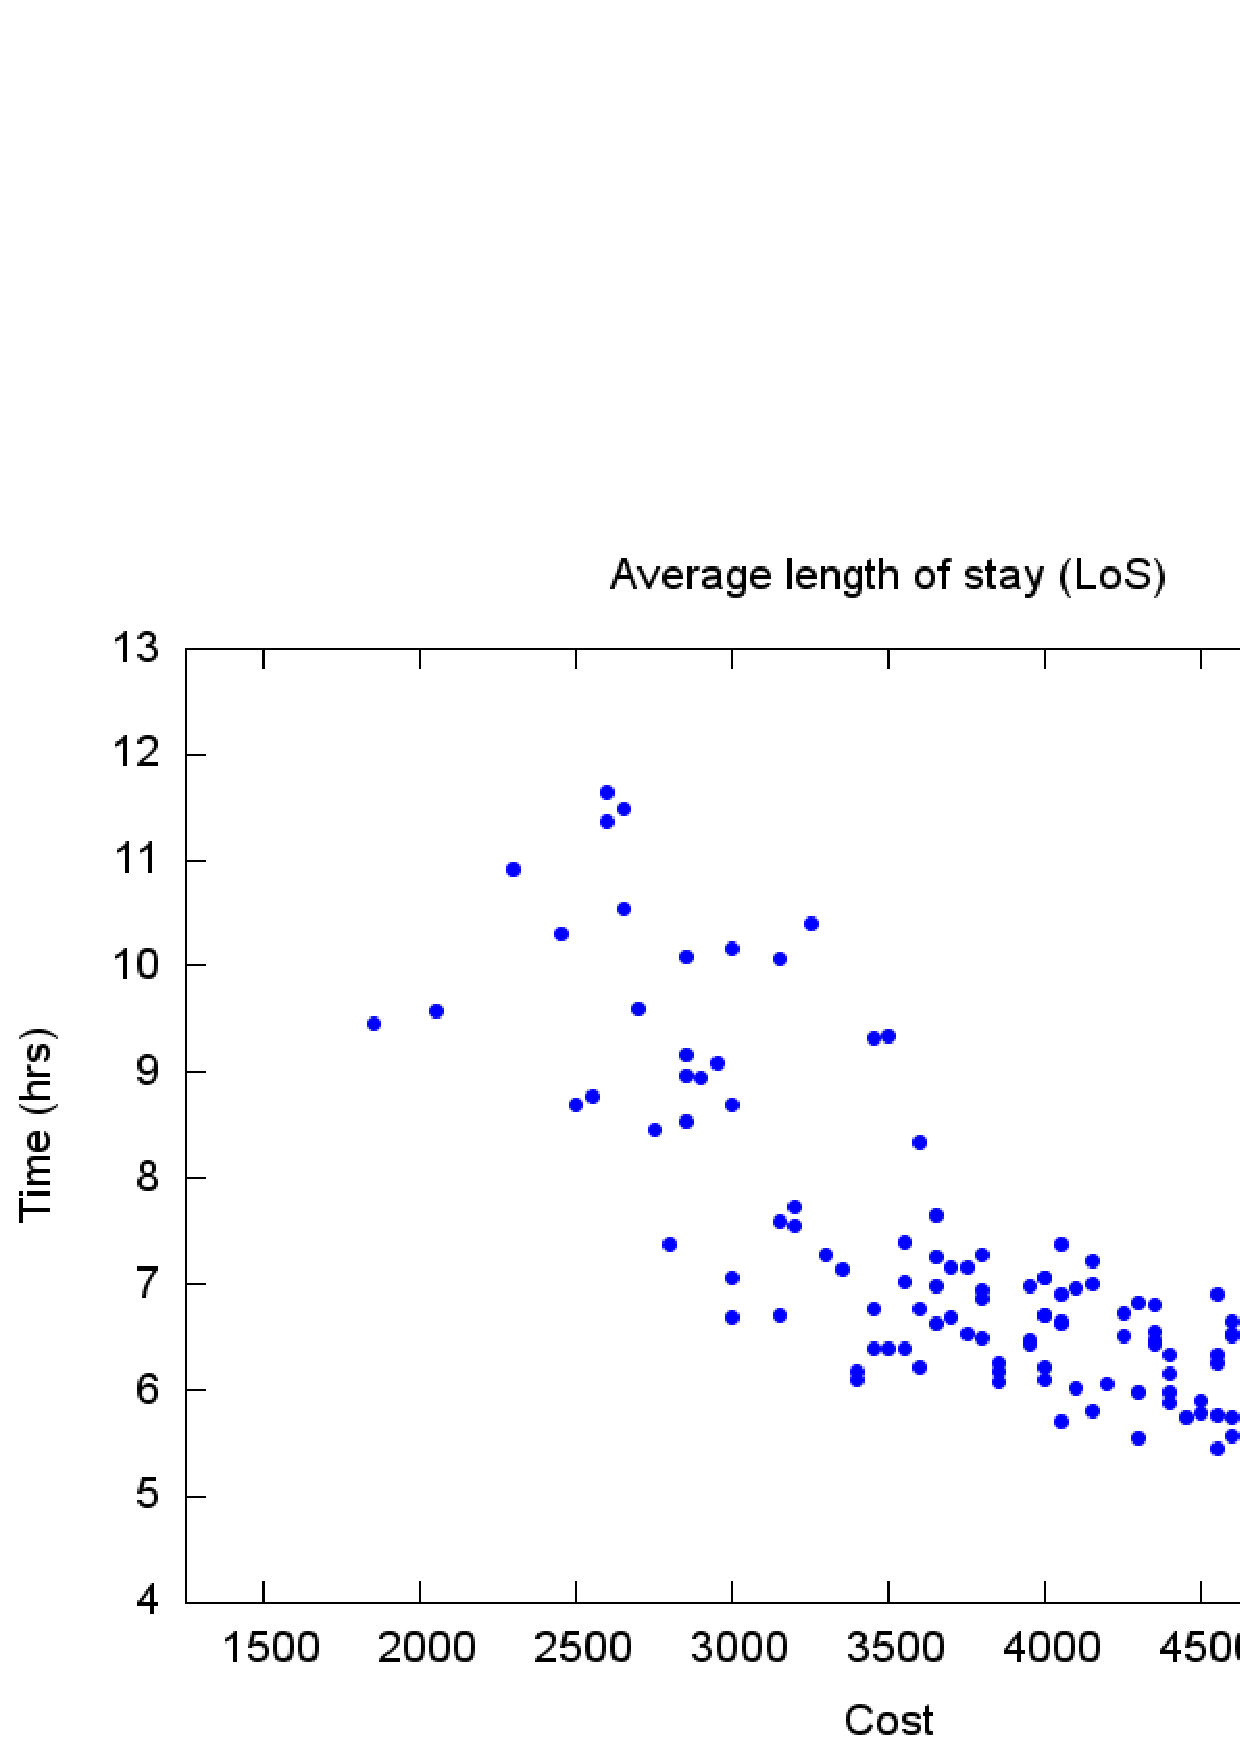
\includegraphics[width=1\columnwidth,height=0.2\paperheight]{figs4/v1\lyxdot 1/MC-518400-23445-100-69-25-150confs-LoS}\caption{Average LoS of 150 configurations obtained by the MC method.\label{subfig:mc16-4}}
\end{figure}
\begin{figure}[H]
\begin{centering}
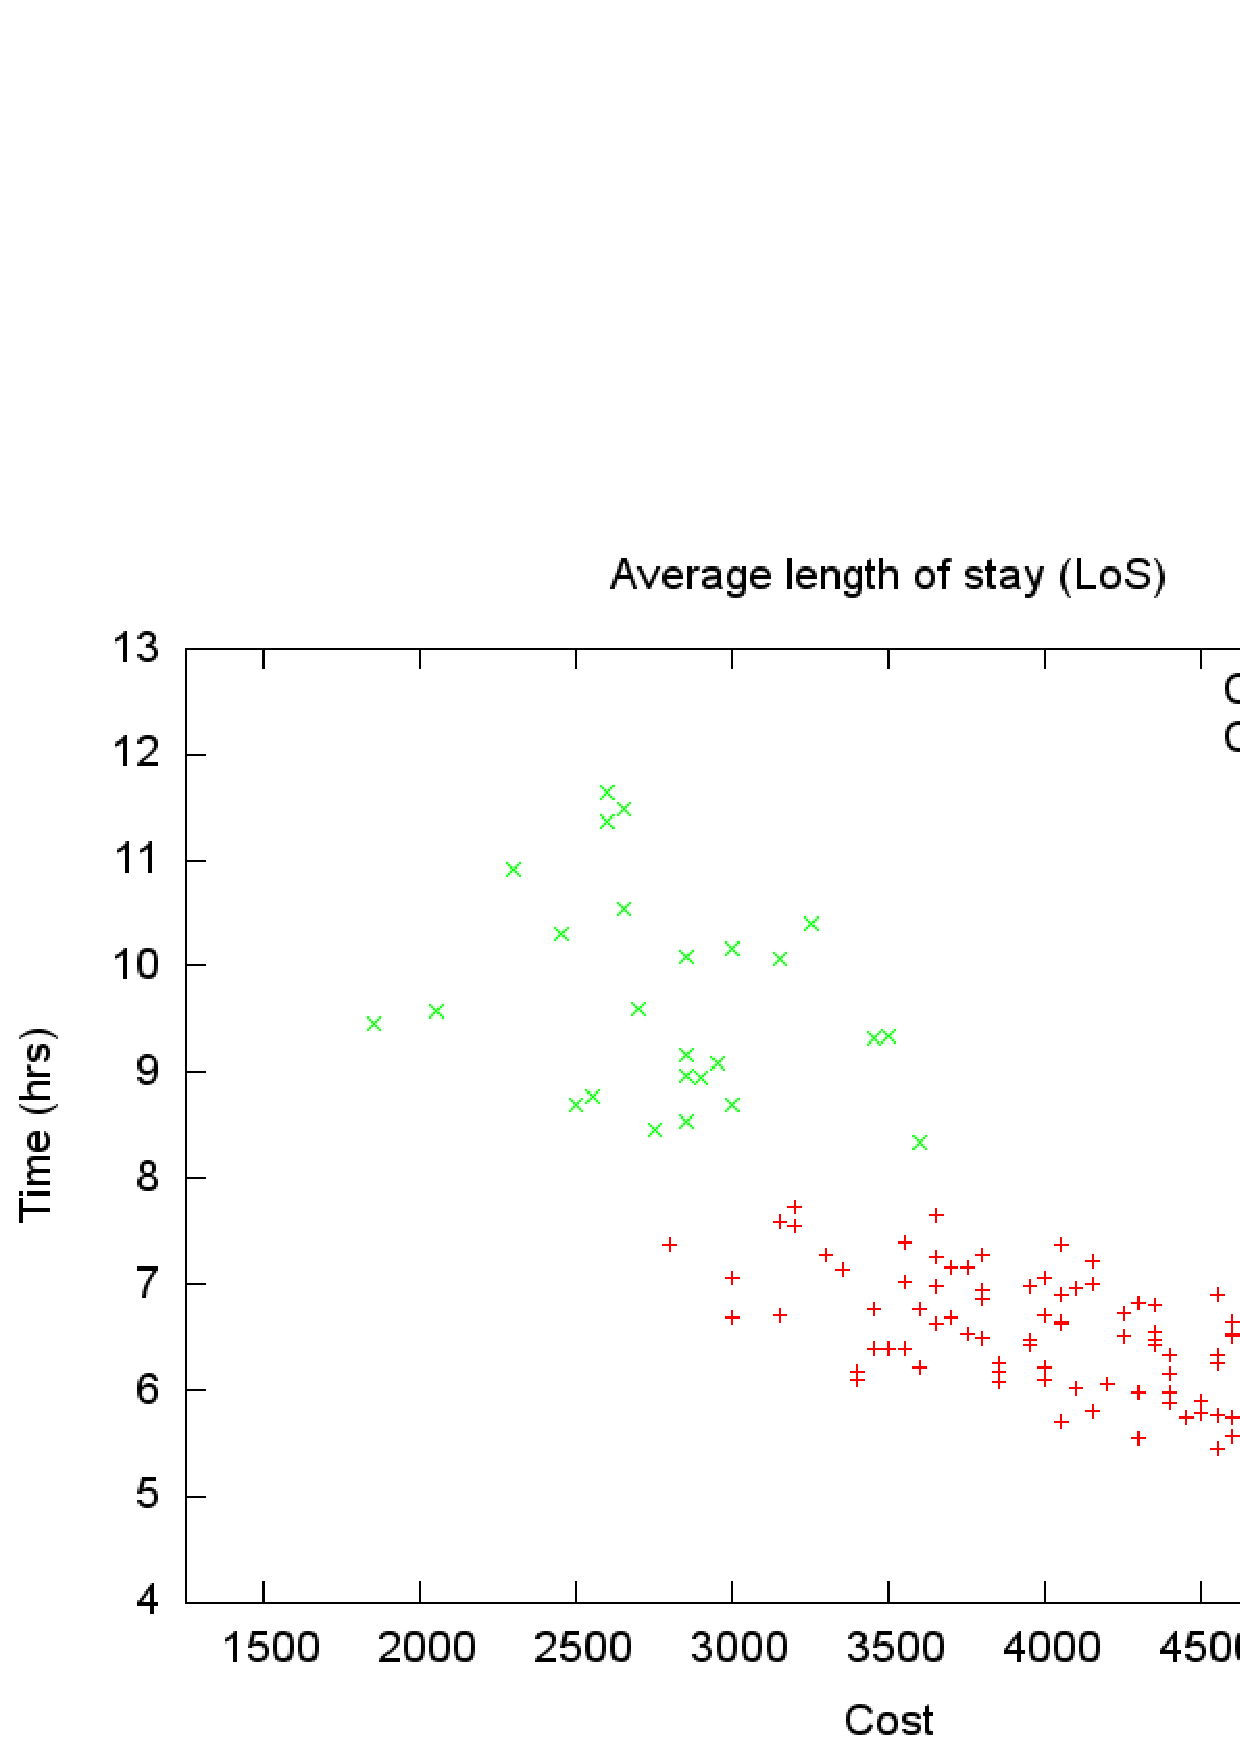
\includegraphics[width=1\columnwidth,height=0.2\paperheight]{figs4/v1\lyxdot 1/K-means-518400-23445-100-69-25-150-Cluster1-125_Cluster2-25}
\par\end{centering}

\caption{The K-means method identified two clusters of average LoS. The red
one delimited the region where the minimum was.\label{subfig:km16-4}}
\end{figure}


\begin{table}[H]
\caption{Optimum staff configurations that got the average minimum LoS for
this workload scenario (up to 17 patients hourly), where S is Senior
and J is Junior. It is shown in red triangle in \ref{subfig:es16-4}.}


\begin{centering}
\begin{tabular}{cc>{\centering}p{1.3cm}ccccc>{\centering}p{2.8cm}}
\hline 
Method & � & LoS (hrs) & D & N & A & EN & XR & Run time (hrs)

256 Pthreads)\tabularnewline
\hline 
ES & 5,500 & 4.6 & 3S,1J & 3J & 2J & 1S & 1J & 4.42\tabularnewline
MC+K-means & 5,500 & 4.6 & 3S,1J & 3J & 2J & 1S & 1J & 0.62\tabularnewline
\hline 
\end{tabular}
\par\end{centering}

\label{tab:16p-d} 
\end{table}


Finally, after applied the MC plus the K-means methods, the \textquotedblleft{}reduced
exhaustive search\textquotedblright{} was performed in such reduced
region identified. The optimum found per each method: the ES, and
the MC plus the K-means methods are presented in \ref{tab:16p-d},
where the sanitary staff configuration (doctors, triage nurses, emergency
nurses, x-ray technicians, and admission personnel), their associated
average minimum LoS, and cost configuration are shown. The two optima
independently found were the same. 


\subsection{Throughput Index}

This objective set was to maximise number of attended patients per
day (Throughput) in the ED, with cost configuration constraint less
or equal to 5,500 �. This index is expressed mathematically in \ref{eq:Throughput index-2}:

\begin{equation}
\begin{aligned} & {\text{Maximise patients attended }} &  & f(D,N,A,En,Xr)\\
 & \text{subject to} &  & D_{cost}+N_{cost}+A_{cost}+En_{cost}+\\
 &  &  & Xr_{cost}\in Cost\leq5,500\:\text{�}
\end{aligned}
\label{eq:Throughput index-2}
\end{equation}


It is worth noting that each of the plotted points for the following
four workload scenarios were obtained running the ED simulator as
many times as points are. Each plotted point corresponds to each of
the 23,445 staff configurations (out of 28,350) that satisfy the cost
restriction.


\subsubsection{First Workload Scenario}

The results of this scenario, up to 4 patients/hour, are shown from
\ref{subfig:es4-5} to \ref{subfig:km4-5}. The ES result is shown
in \ref{subfig:es4-5}, where the red triangles were the maximum. 

The MC plus the K-means methods results are shown in \ref{subfig:mc4-5}
to \ref{subfig:km4-5}, respectively. The MC method found 1,325 configurations.
However, it was difficult to get any conclusion about such region;
therefore, the complementary K-means method was performed. The K-means
method identified two different clusters, shown in \ref{subfig:km4-5},
the most important was the green cluster, which delimited the region
where the optimum were.

\begin{comment}
The graphics \ref{subfloat:pipe4} and \ref{subfloat:contour4} shown
another way to visualise the connectivity characteristic of the reduced
regions found by the AP, and the MC plus the K-means methods. In such
connected reduced regions the ``reduced exhaustive search'' is applied.
The axes of such graphs are the first column of \ref{subtab:As-pipe},
\ref{subtab:Ns-pipe}, and \ref{subtab:Ds-pipe}, where they were
ordered by the pipeline approach (PA) \ref{eq:Pipeline formula}.
\end{comment}
\begin{comment}
\begin{figure}[H]
\noindent \begin{centering}
\begin{minipage}[t]{0.45\linewidth}%
\noindent \begin{center}
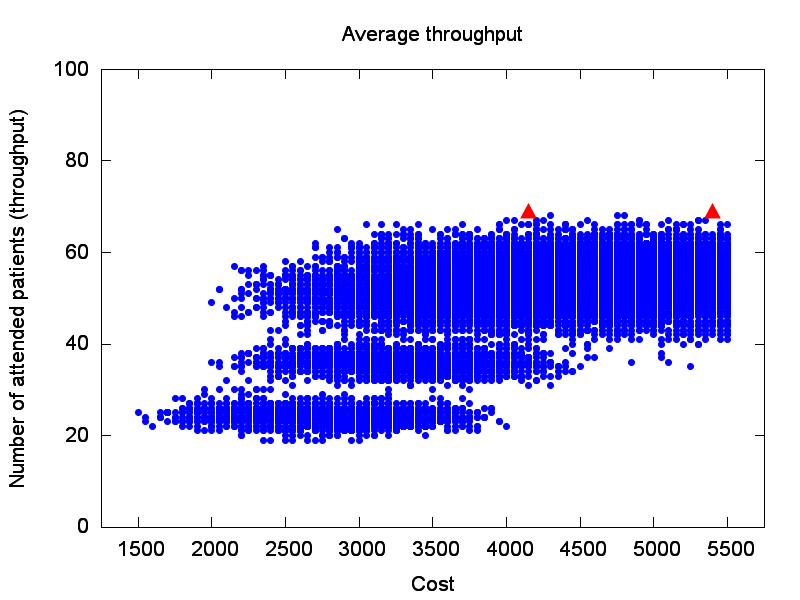
\includegraphics[width=1\columnwidth]{figs4/v1.2/v1-25-exh-throughput-max.png}
\par\end{center}

\noindent \begin{center}
\caption{}

\par\end{center}%
\end{minipage}
\par\end{centering}

\noindent \begin{centering}
\vfill{}

\par\end{centering}

\begin{minipage}[t]{0.45\textwidth}%
\noindent \begin{center}
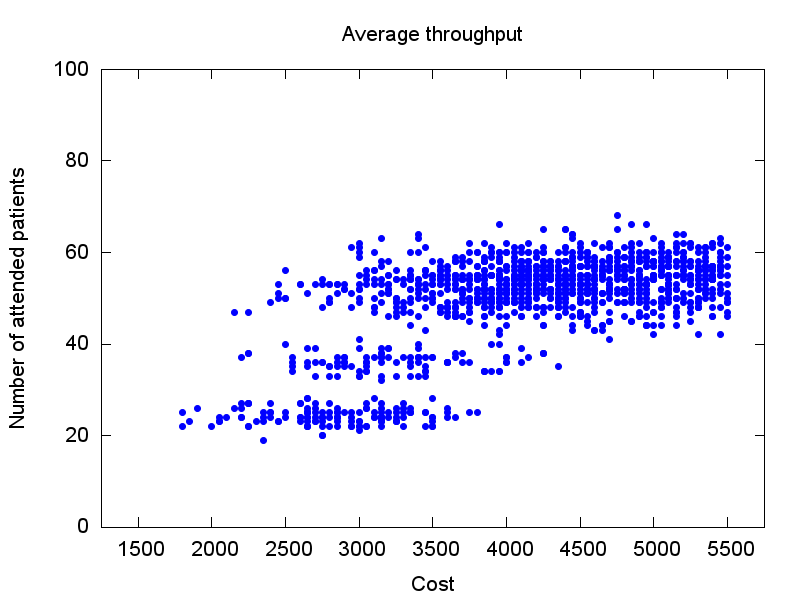
\includegraphics[width=1\columnwidth]{figs4/v1.2/MC-518400-23445-25-69-25-1325confs-Throughput.png}
\par\end{center}

\caption{}
%
\end{minipage}\hfill{}%
\begin{minipage}[t]{0.45\textwidth}%
\noindent \begin{center}
\includegraphics[width=1\columnwidth]{figs4/v1.2/K-means-518400-23445-25-69-25-1325-Cluster1-555_Cluster2-737.png}
\par\end{center}

\caption{}
%
\end{minipage}
\end{figure}
\end{comment}


Finally, after applied the MC plus the K-means methods, the \textquotedblleft{}reduced
exhaustive search\textquotedblright{} was performed in such reduced
region identified. The optimum found per each method: the ES and the
MC plus the K-means methods are presented in \ref{tab:4p-e}, where
the sanitary staff configuration (doctors, triage nurses, emergency
nurses, x-ray technicians, and admission personnel), their associated
average maximum Throughput, and cost configuration are shown. The
two optima independently found were the same. 
\begin{figure}[H]
\centering{}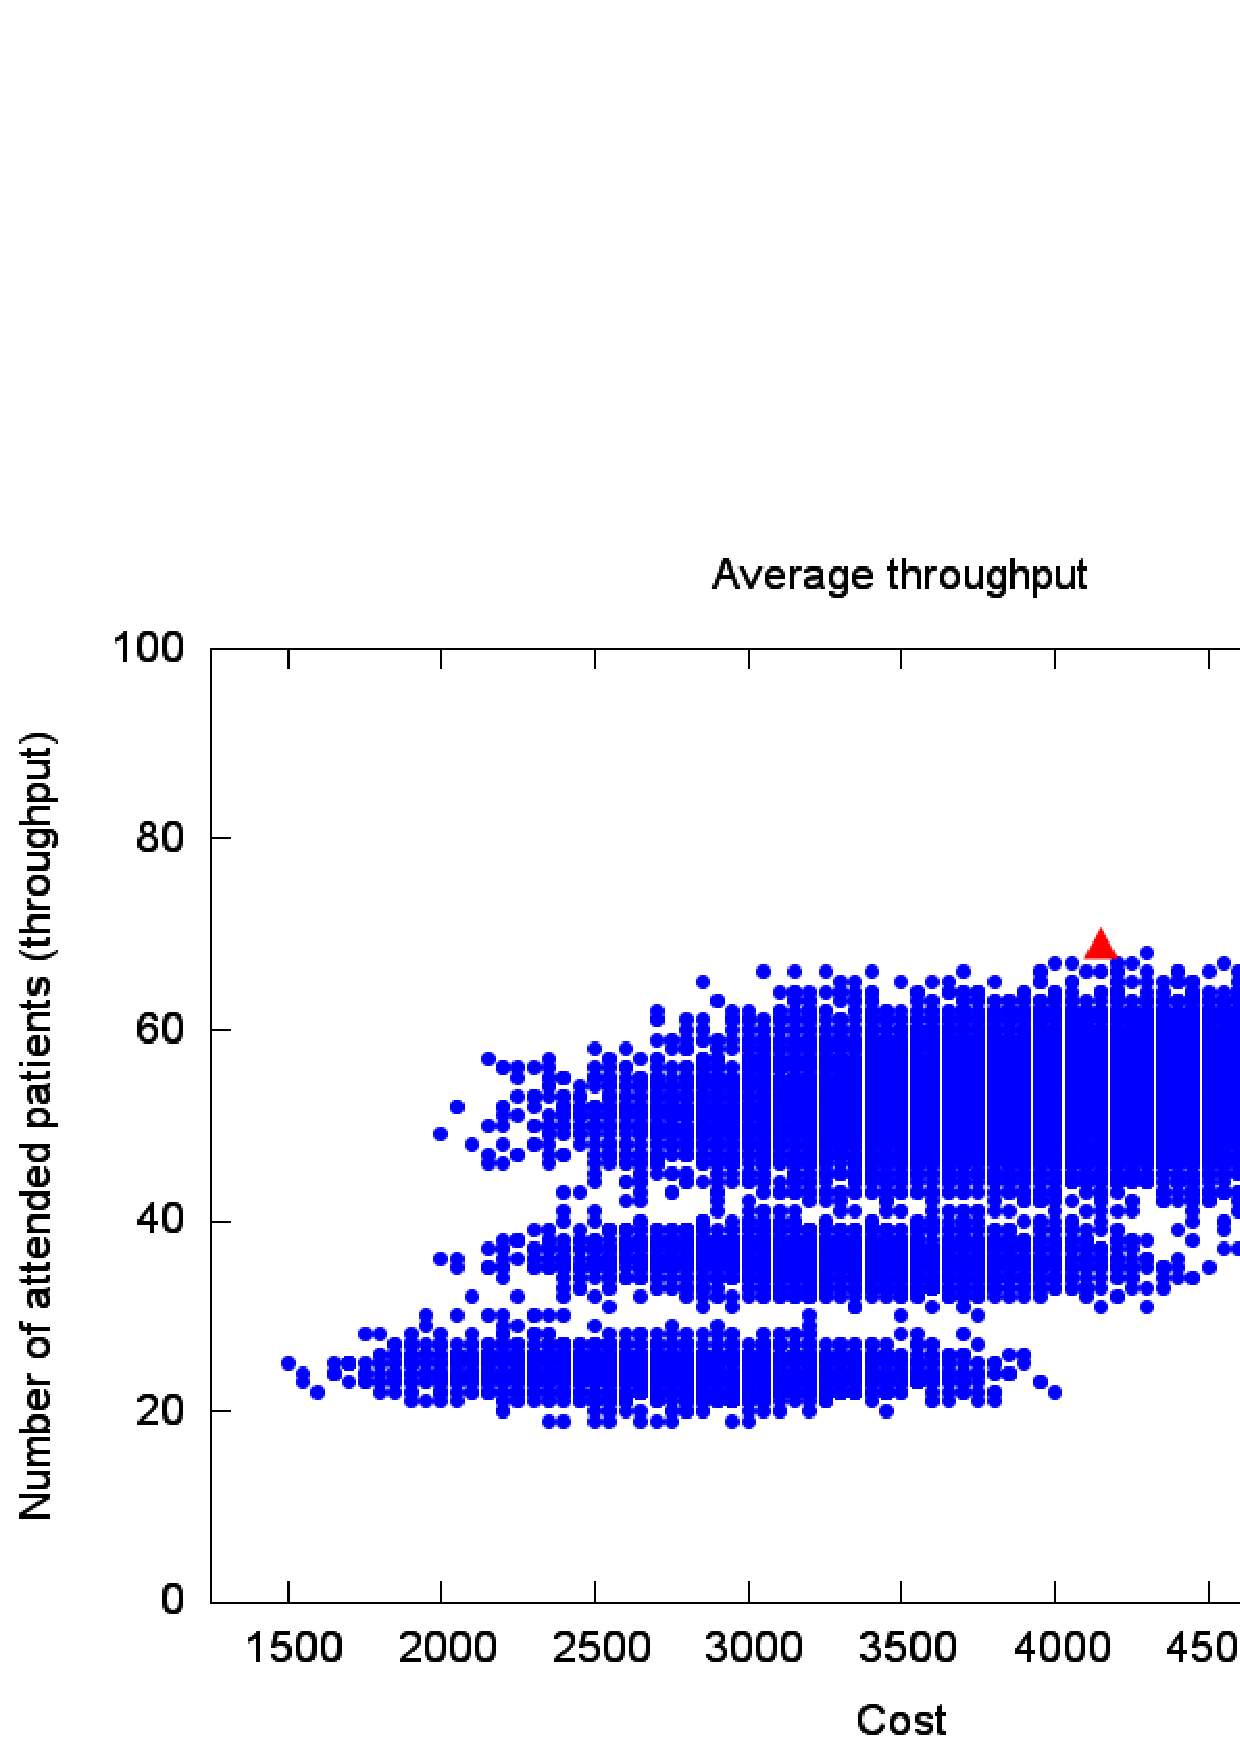
\includegraphics[width=1\columnwidth,height=0.19\paperheight]{figs4/v1\lyxdot 2/v1-25-exh-throughput-max}\caption{Average number of attended patients obtained by the ES method. The
red triangles were the maxima. \label{subfig:es4-5}}
\end{figure}
\begin{figure}[H]
\centering{}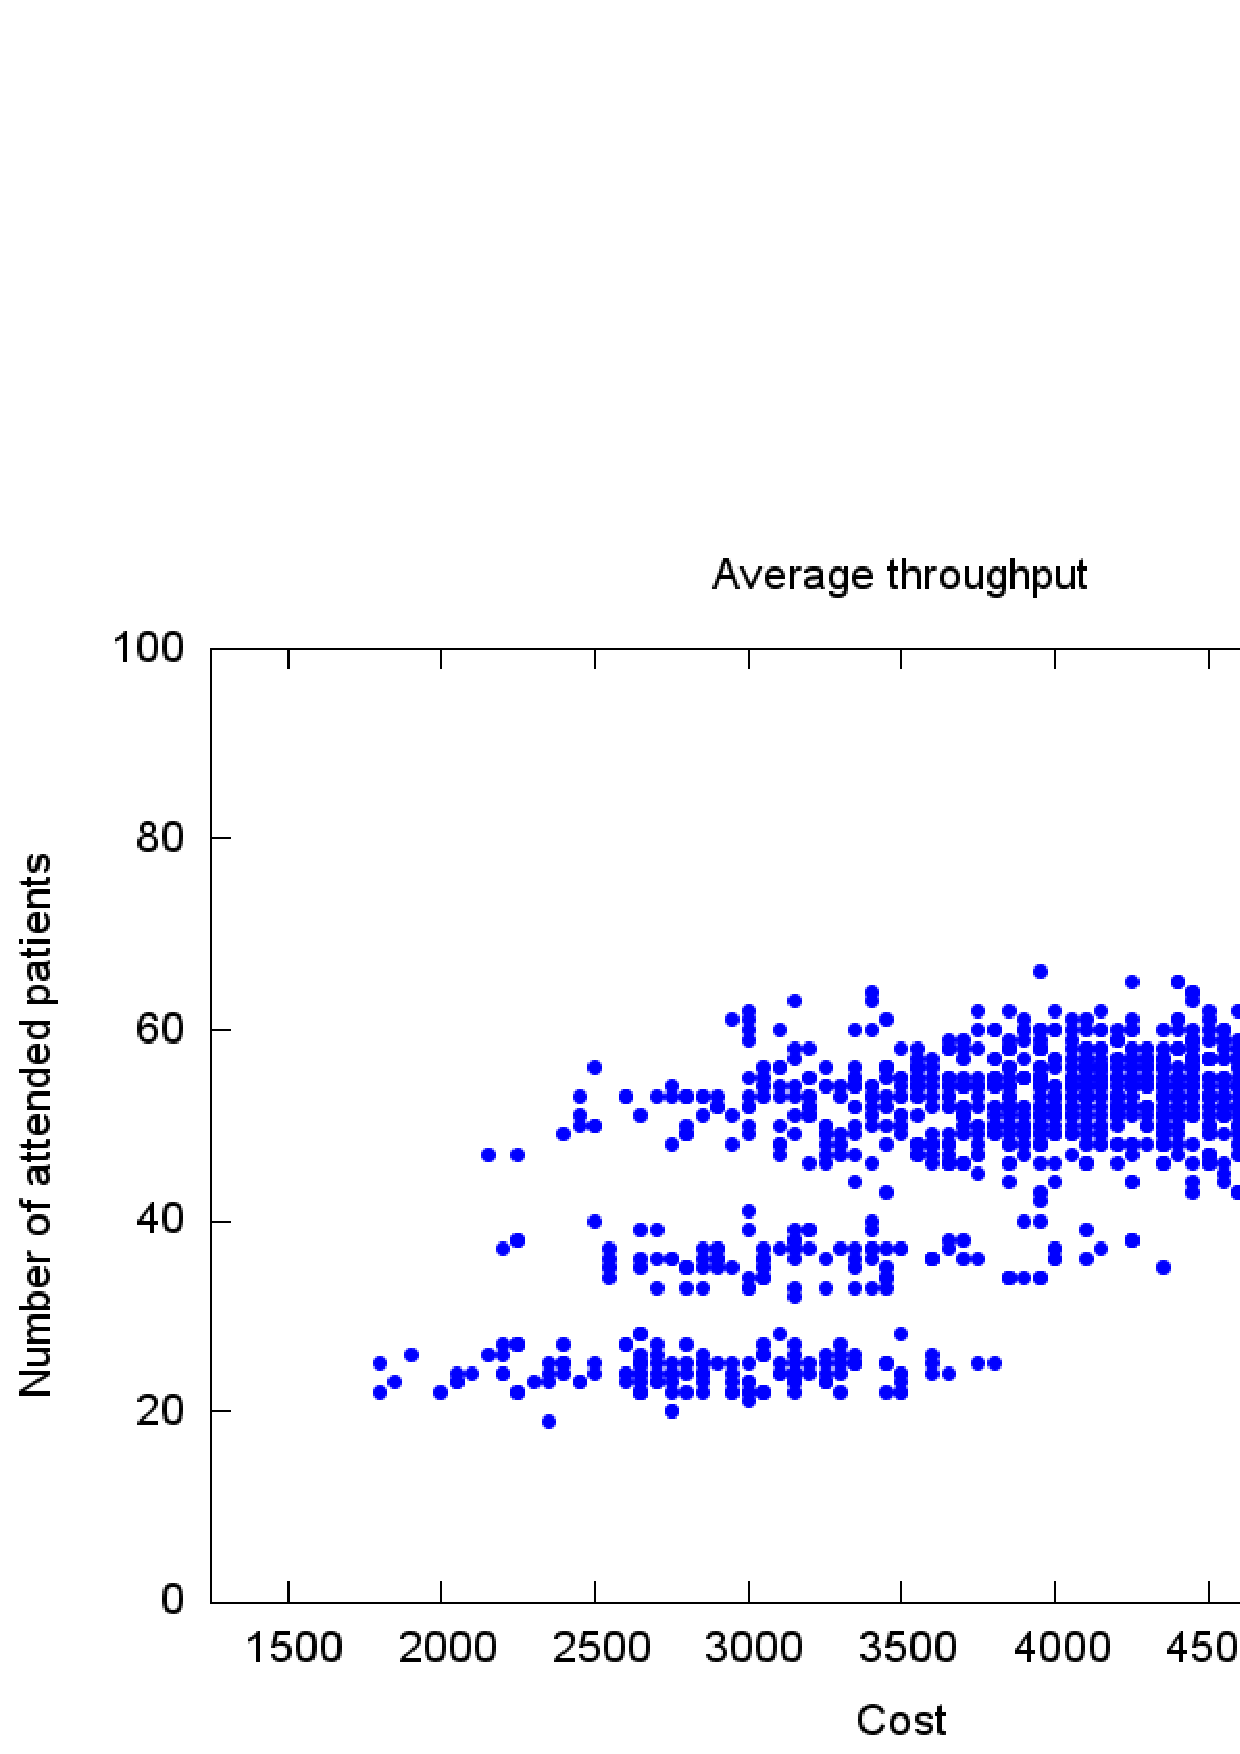
\includegraphics[width=1\columnwidth,height=0.19\paperheight]{figs4/v1\lyxdot 2/MC-518400-23445-25-69-25-1325confs-Throughput}\caption{Average number of attended patients of 1,325 configurations obtained
by the MC method.\label{subfig:mc4-5}}
\end{figure}
\begin{figure}[H]
\begin{centering}
\includegraphics[width=1\columnwidth,height=0.19\paperheight]{figs4/v1\lyxdot 2/K-means-518400-23445-25-69-25-1325-Cluster1-555_Cluster2-737}
\par\end{centering}

\caption{The K-means method identified two clusters of average number of attended
patients. The green one delimited the region where the maxima were.
\label{subfig:km4-5}}
\end{figure}


\begin{table}[H]
\caption{Optimum staff configurations that got the average maximum Throughput
for this workload scenario (up to 4 patients hourly), where S is Senior
and J is Junior. These optimum sanitary staff configurations are shown
in red triangle in \ref{subfig:es4-5}.}


\begin{centering}
\begin{tabular}{cc>{\centering}p{1.8cm}ccccc>{\centering}p{2.8cm}}
\hline 
Method & � & \#attended patients & D & N & A & EN & XR & Run time (hrs)

256 Pthreads)\tabularnewline
\hline 
ES & 4,150 & 69 & 2S & 2S & 1S,2J  & 1S & 1J & 2.54\tabularnewline
MC+K-means & 4,150 & 69 & 2S & 2S & 1S,2J  & 1S & 1J & 0.79\tabularnewline
\hline 
\end{tabular}
\par\end{centering}

\label{tab:4p-e}
\end{table}



\subsubsection{Second Workload Scenario}

The results of this scenario, up to 9 patients/hour, are shown from
\ref{subfig:es8-5} to \ref{subfig:km8-5}. The ES result is shown
in \ref{subfig:es8-5}, where the red triangle was the maximum. 

The MC plus the K-means methods results are shown in \ref{subfig:mc8-5}
to \ref{subfig:km8-5}, respectively. The MC method found 1,350 configurations.
However, it was difficult to get any conclusion about such region;
therefore, the complementary K-means method was performed. The K-means
method identified two different clusters, shown in \ref{subfig:km8-5},
the most important was the green cluster, which delimited the region
where the optimum was.

\begin{comment}
The graphics \ref{subfloat:pipe4} and \ref{subfloat:contour4} shown
another way to visualise the connectivity characteristic of the reduced
regions found by the AP, and the MC plus the K-means methods. In such
connected reduced regions the ``reduced exhaustive search'' is applied.
The axes of such graphs are the first column of \ref{subtab:As-pipe},
\ref{subtab:Ns-pipe}, and \ref{subtab:Ds-pipe}, where they were
ordered by the pipeline approach (PA) \ref{eq:Pipeline formula}.
\end{comment}
\begin{comment}
\begin{figure}[H]
\noindent \begin{centering}
\begin{minipage}[t]{0.45\linewidth}%
\noindent \begin{center}
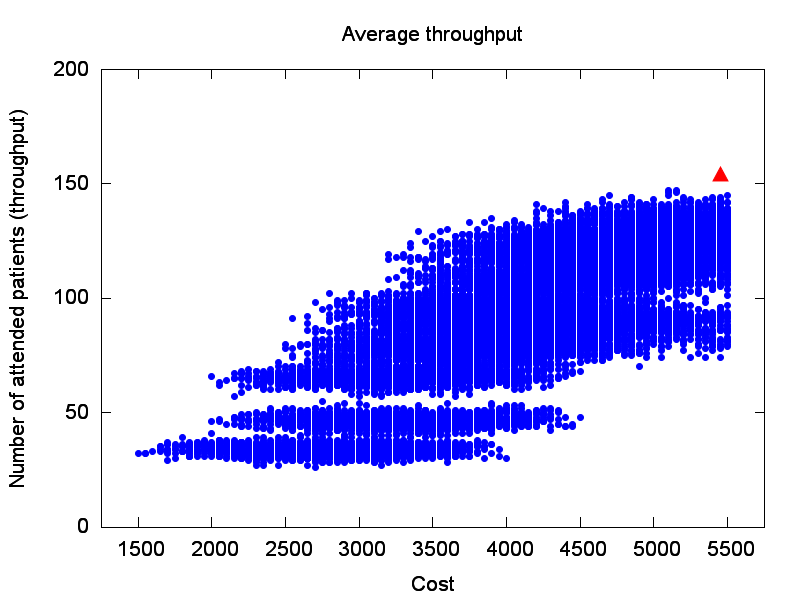
\includegraphics[width=1\columnwidth]{figs4/v1.2/v1-50-exh-throughput-max.png}
\par\end{center}

\noindent \begin{center}
\caption{Average number of attended patients obtained by the ES method. The
red triangle was the maximum.}

\par\end{center}%
\end{minipage}
\par\end{centering}

\noindent \begin{centering}
\vfill{}

\par\end{centering}

\begin{minipage}[t]{0.45\textwidth}%
\noindent \begin{center}
\includegraphics[width=1\columnwidth]{figs4/v1.2/MC-518400-23445-50-69-25-1350confs-Throughput.png}
\par\end{center}

\caption{}
%
\end{minipage}\hfill{}%
\begin{minipage}[t]{0.45\textwidth}%
\noindent \begin{center}
\includegraphics[width=1\columnwidth]{figs4/v1.2/K-means-518400-23445-50-69-25-1350-Cluster1-564_Cluster2-752.png}
\par\end{center}

\caption{}
%
\end{minipage}
\end{figure}
\end{comment}


Finally, after applied the MC plus the K-means methods, the \textquotedblleft{}reduced
exhaustive search\textquotedblright{} was performed in such reduced
region identified. The optimum found per each method: the ES and the
MC plus the K-means methods are presented in \ref{tab:8p-e}, where
the sanitary staff configuration (doctors, triage nurses, emergency
nurses, x-ray technicians, and admission personnel), their associated
average maximum Throughput, and cost configuration are shown. The
two optima independently found were the same. 
\begin{figure}[H]
\centering{}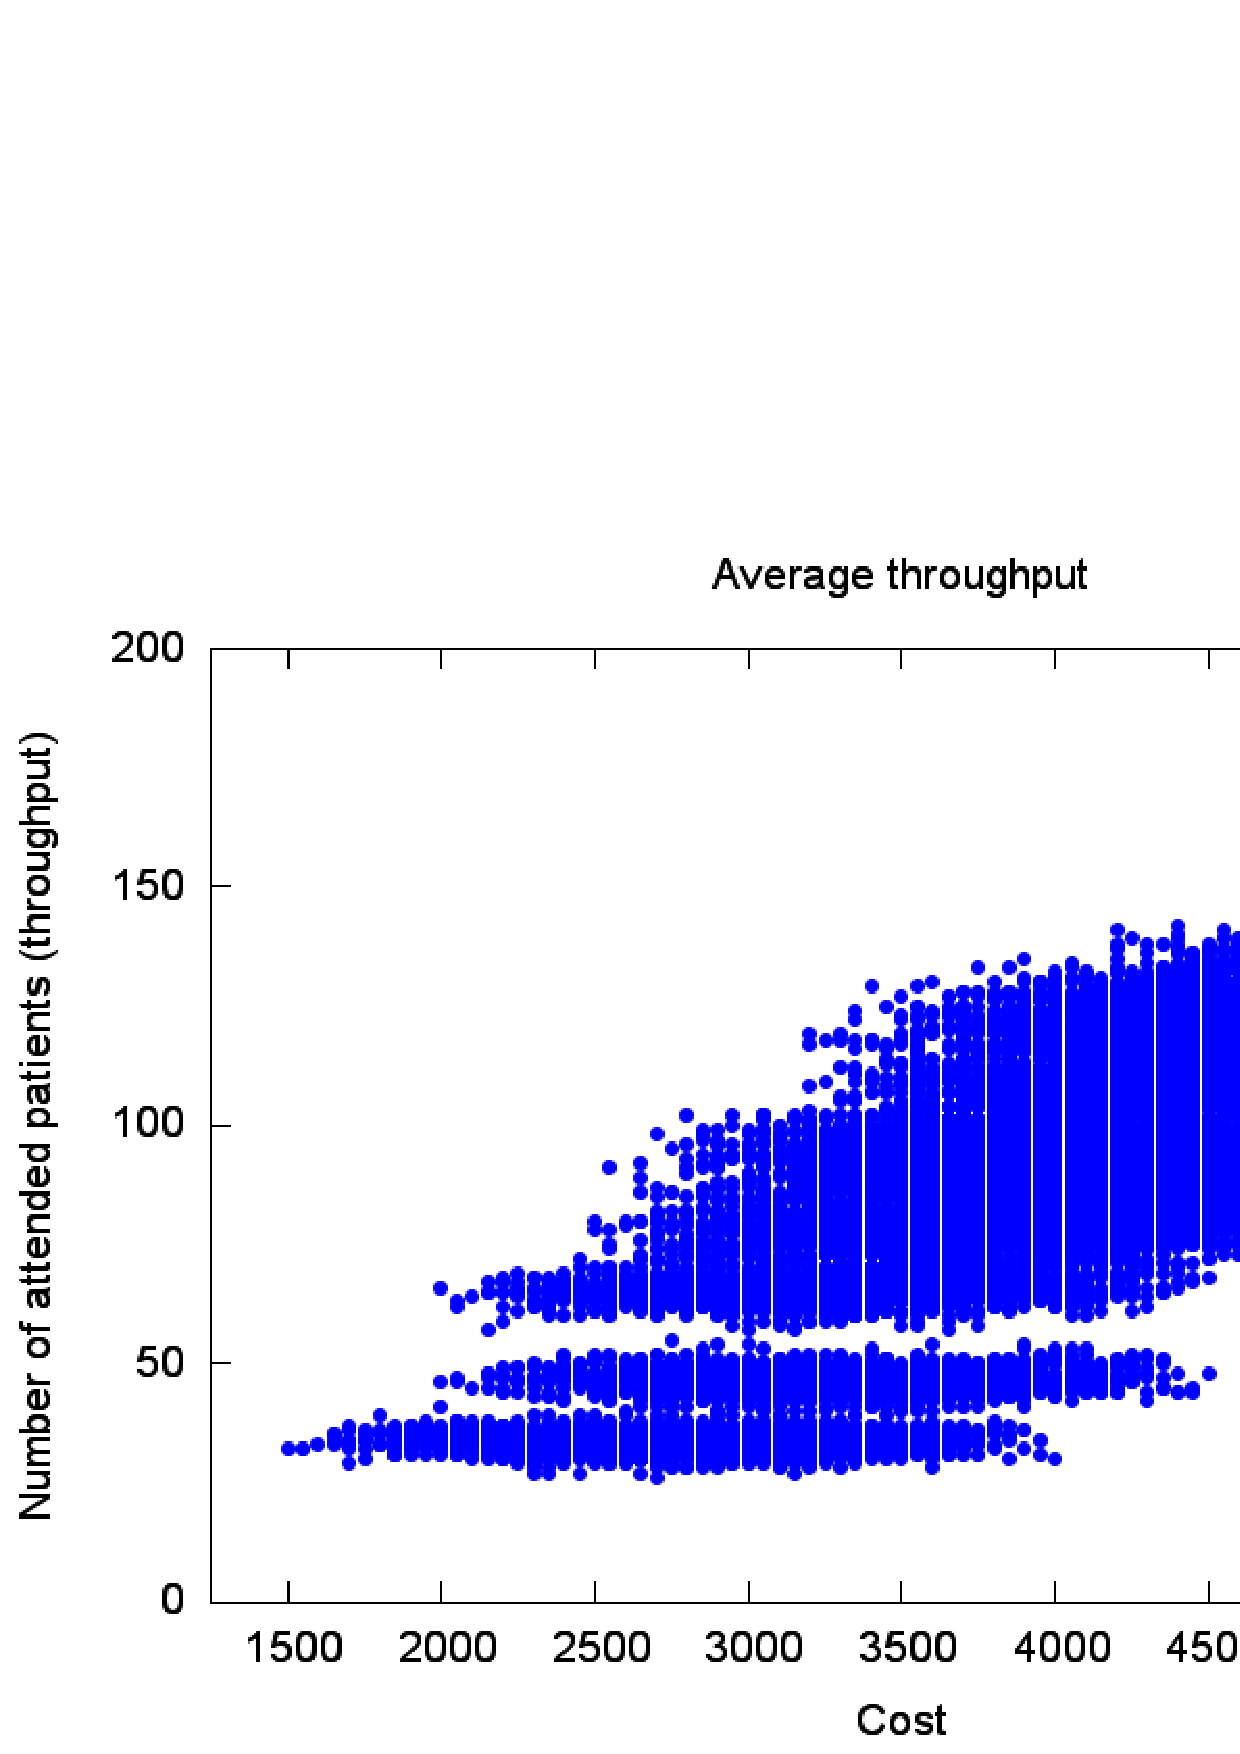
\includegraphics[width=1\columnwidth,height=0.2\paperheight]{figs4/v1\lyxdot 2/v1-50-exh-throughput-max}\caption{Average number of attended patients obtained by the ES method. The
red triangle was the maximum. \label{subfig:es8-5}}
\end{figure}
\begin{figure}[H]
\centering{}\includegraphics[width=1\columnwidth,height=0.2\paperheight]{figs4/v1\lyxdot 2/MC-518400-23445-50-69-25-1350confs-Throughput}\caption{Average number of attended patients of 1,350 configurations obtained
by the MC method.\label{subfig:mc8-5}}
\end{figure}
\begin{figure}[H]
\begin{centering}
\includegraphics[width=1\columnwidth,height=0.2\paperheight]{figs4/v1\lyxdot 2/K-means-518400-23445-50-69-25-1350-Cluster1-564_Cluster2-752}
\par\end{centering}

\caption{The K-means method identified two clusters of average number of attended
patients. The green one delimited the region where the maximum was.\label{subfig:km8-5}}
\end{figure}


\begin{table}[H]
\caption{Optimum staff configurations that got the average maximum Throughput
for this workload scenario (up to 9 patients hourly), where S is Senior
and J is Junior. These optimum sanitary staff configurations are shown
in red triangle in \ref{subfig:es8-5}.}


\begin{centering}
\begin{tabular}{cc>{\centering}p{1.8cm}ccccc>{\centering}p{2.8cm}}
\hline 
Method & � & \#attended patients & D & N & A & EN & XR & Run time (hrs)

256 Pthreads)\tabularnewline
\hline 
ES & 5,450 & 154 & 2S,2J & 2S & 2S & 1S,1J & 1S & 3.07\tabularnewline
MC+K-means & 5,450 & 154 & 2S,2J & 2S & 2S & 1S,1J & 1S & 0.7\tabularnewline
\hline 
\end{tabular}
\par\end{centering}

\label{tab:8p-e} 
\end{table}


\clearpage{}


\subsubsection{Third Workload Scenario}

The results of this scenario, up to 13 patients/hour, are shown from
\ref{subfig:es12-5} to \ref{subfig:km12-5}. The ES result is shown
in \ref{subfig:es12-5}, where the red triangle was the maximum. 
\begin{figure}[H]
\centering{}\includegraphics[width=1\columnwidth,height=0.2\paperheight]{figs4/v1\lyxdot 2/v1-75-exh-throughput-max}\caption{Average number of attended patients obtained by the ES method. The
red triangle was the maximum.\label{subfig:es12-5}}
\end{figure}


The MC plus the K-means methods results are shown in \ref{subfig:mc12-5}
to \ref{subfig:km12-5}, respectively. The MC method found 1,100 configurations.
\begin{figure}[H]
\centering{}\includegraphics[width=1\columnwidth,height=0.2\paperheight]{figs4/v1\lyxdot 2/MC-518400-23445-75-69-25-1100confs-Throughput}\caption{Average number of attended patients of 1,110 configurations obtained
by the MC method.\label{subfig:mc12-5}}
\end{figure}
However, it was difficult to get any conclusion about such region;
therefore, the complementary K-means method was performed. The K-means
method identified two different clusters, shown in \ref{subfig:km12-5},
the most important was the green cluster, which delimited the region
where the optimum was.
\begin{figure}[H]
\begin{centering}
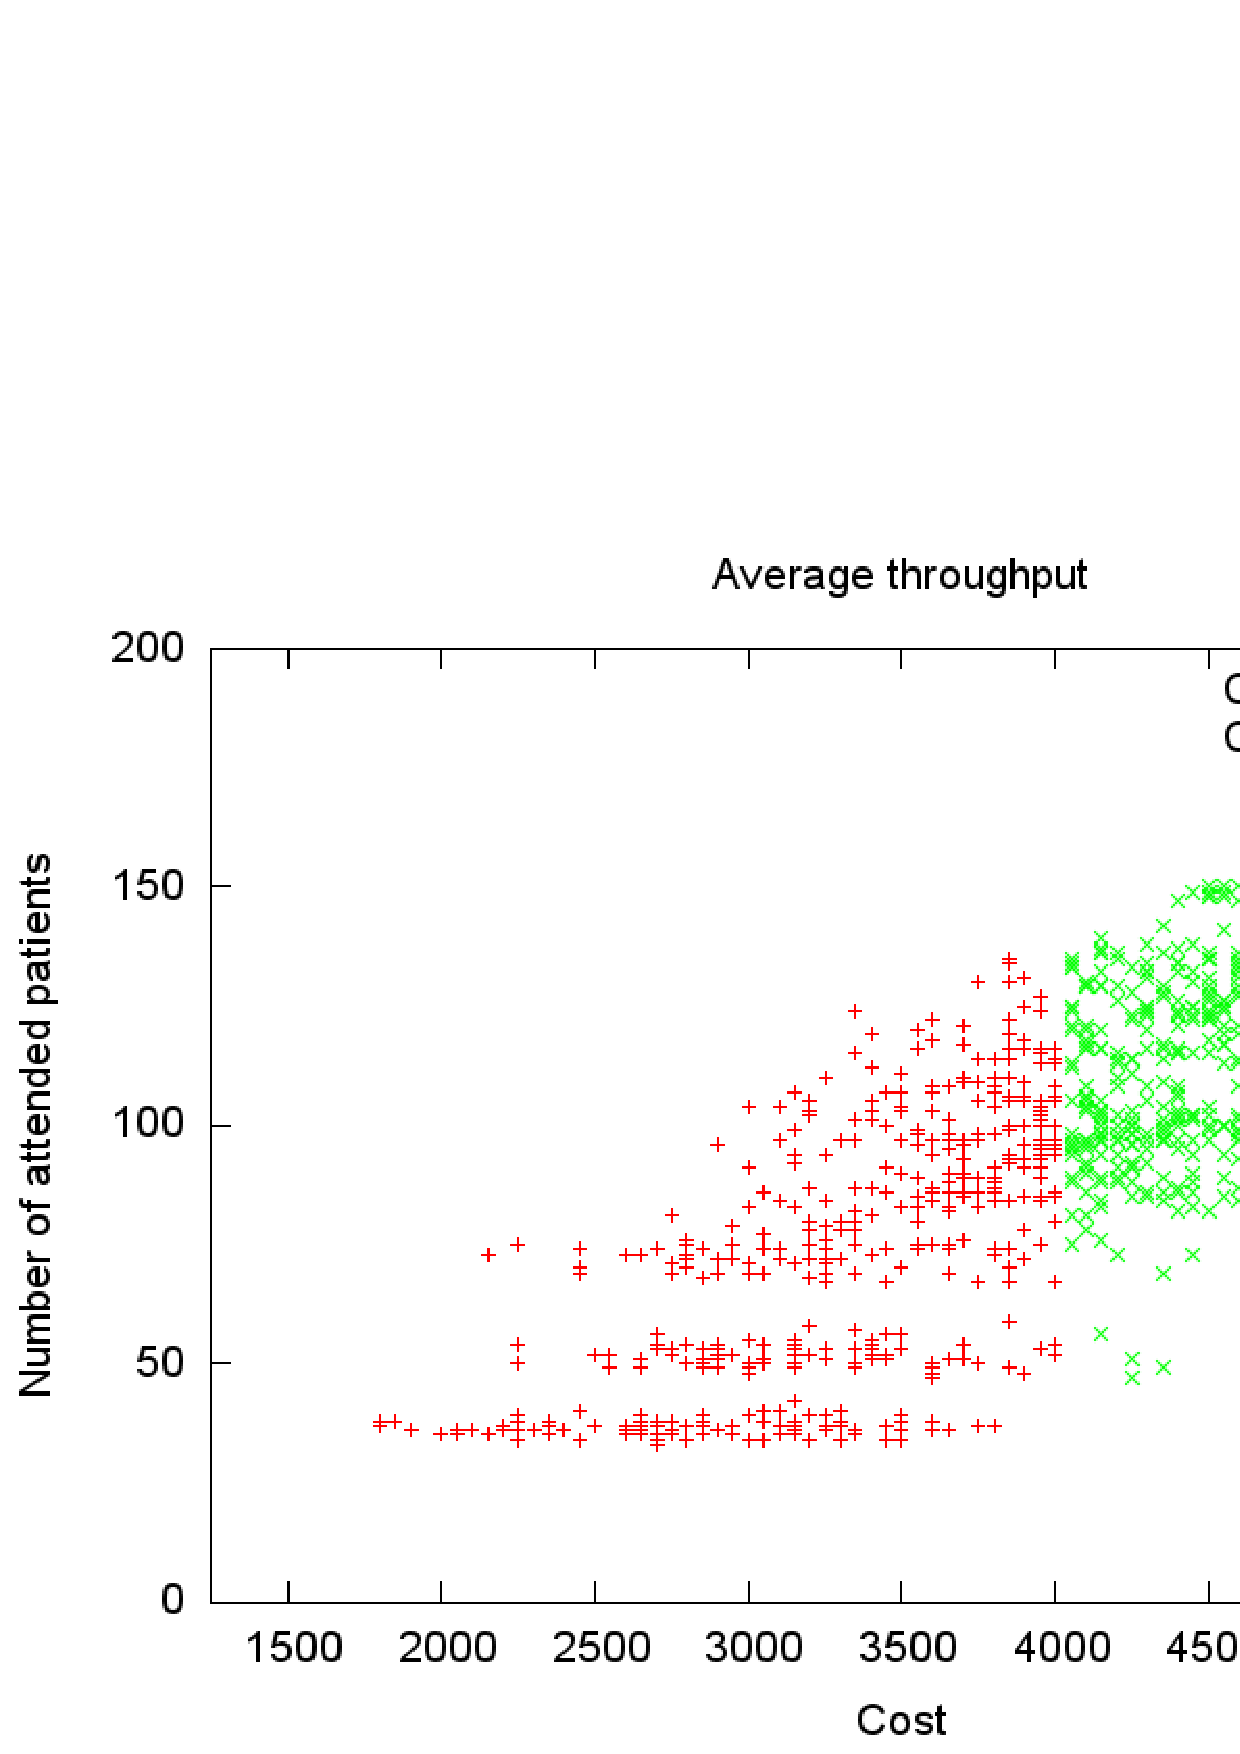
\includegraphics[width=1\columnwidth,height=0.2\paperheight]{figs4/v1\lyxdot 2/K-means-518400-23445-75-69-25-1100-Cluster1-458_Cluster2-619}
\par\end{centering}

\caption{The K-means method identified two clusters of average number of attended
patients. The green one delimited the region where the maximum was.\label{subfig:km12-5}}
\end{figure}


\begin{comment}
The graphics \ref{subfloat:pipe4} and \ref{subfloat:contour4} shown
another way to visualise the connectivity characteristic of the reduced
regions found by the AP, and the MC plus the K-means methods. In such
connected reduced regions the ``reduced exhaustive search'' is applied.
The axes of such graphs are the first column of \ref{subtab:As-pipe},
\ref{subtab:Ns-pipe}, and \ref{subtab:Ds-pipe}, where they were
ordered by the pipeline approach (PA) \ref{eq:Pipeline formula}.
\end{comment}
\begin{comment}
\begin{figure}[H]
\noindent \begin{centering}
\begin{minipage}[t]{0.45\linewidth}%
\noindent \begin{center}
\includegraphics[width=1\columnwidth]{figs4/v1.2/v1-75-exh-throughput-max.png}
\par\end{center}

\noindent \begin{center}
\caption{}

\par\end{center}%
\end{minipage}
\par\end{centering}

\noindent \begin{centering}
\vfill{}

\par\end{centering}

\begin{minipage}[t]{0.45\textwidth}%
\noindent \begin{center}
\includegraphics[width=1\columnwidth]{figs4/v1.2/MC-518400-23445-75-69-25-1100confs-Throughput.png}
\par\end{center}

\caption{}
%
\end{minipage}\hfill{}%
\begin{minipage}[t]{0.45\textwidth}%
\noindent \begin{center}
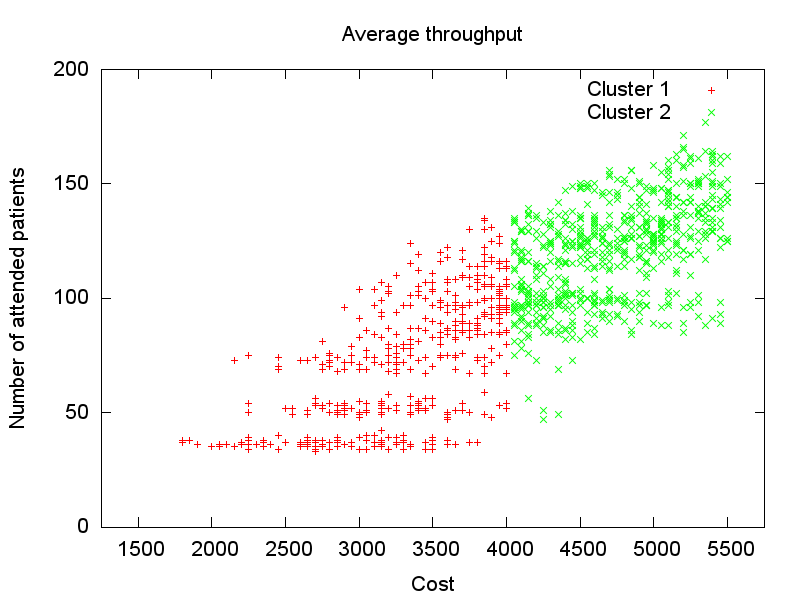
\includegraphics[width=1\columnwidth]{figs4/v1.2/K-means-518400-23445-75-69-25-1100-Cluster1-458_Cluster2-619.png}
\par\end{center}

\caption{}
%
\end{minipage}
\end{figure}
\end{comment}


Finally, after applied the MC plus the K-means methods, the \textquotedblleft{}reduced
exhaustive search\textquotedblright{} was performed in such reduced
region identified. The optimum found per each method: the ES and the
MC plus the K-means methods are presented in \ref{tab:12p-e}, where
the sanitary staff configuration (doctors, triage nurses, emergency
nurses, x-ray technicians, and admission personnel), their associated
average maximum Throughput, and cost configuration are shown. The
two optima independently found were the same. 

\begin{table}[H]
\caption{Optimum staff configurations that got the average maximum Throughput
for this workload scenario (up to 13 patients hourly), where S is
Senior and J is Junior. These optimum sanitary staff configurations
are shown in red triangle in \ref{subfig:es12-5}.}


\begin{centering}
\begin{tabular}{cc>{\centering}p{1.8cm}ccccc>{\centering}p{2.8cm}}
\hline 
Method & � & \#attended patients & D & N & A & EN & XR & Run time (hrs)

256 Pthreads)\tabularnewline
\hline 
ES & 5,450 & 178 & 3S,1J & 2S & 2S & 1S,1J & 1S & 3.7\tabularnewline
MC+K-means & 5,450 & 178 & 3S,1J & 2S & 2S & 1S,1J & 1S & 0.85\tabularnewline
\hline 
\end{tabular}
\par\end{centering}

\label{tab:12p-e} 
\end{table}



\subsubsection{Four Workload Scenario}

The results of this scenario, up to 17 patients/hour, are shown from
\ref{subfig:es16-5} to \ref{subfig:km16-5}. The ES result is shown
in \ref{subfig:es16-5}, where the red triangle was the maximum. 

The MC plus the K-means methods results are shown in \ref{subfig:mc16-5}
to \ref{subfig:km16-5}, respectively. The MC method found 1,225 configurations.
However, it was difficult to get any conclusion about such region;
therefore, the complementary K-means method was performed. The K-means
method identified two different clusters, shown in \ref{subfig:km16-5},
the most important was the green cluster, which delimited the region
where the optimum was.
\begin{figure}[H]
\centering{}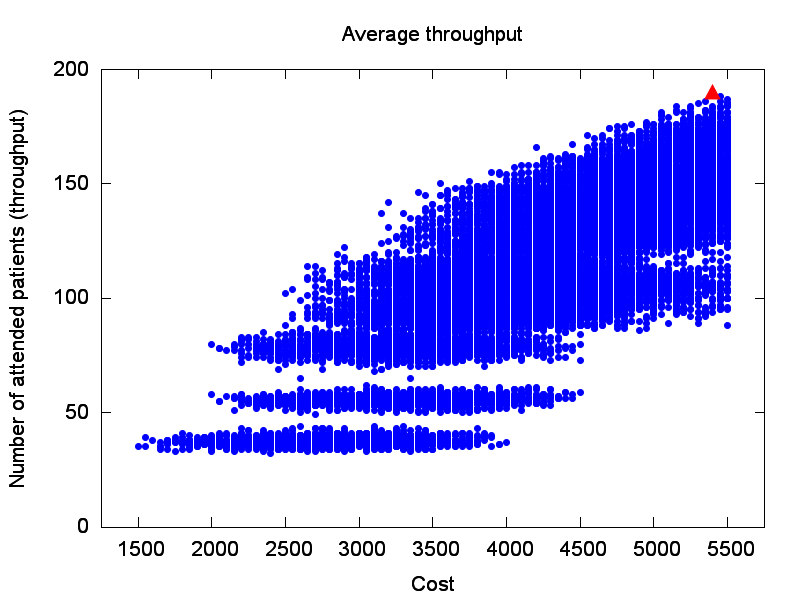
\includegraphics[width=1\columnwidth,height=0.19\paperheight]{figs4/v1\lyxdot 2/v1-100-exh-throughput-max}\caption{Average number of attended patients obtained by the ES method. The
red triangle was the maximum.\label{subfig:es16-5}}
\end{figure}
\begin{figure}[H]
\centering{}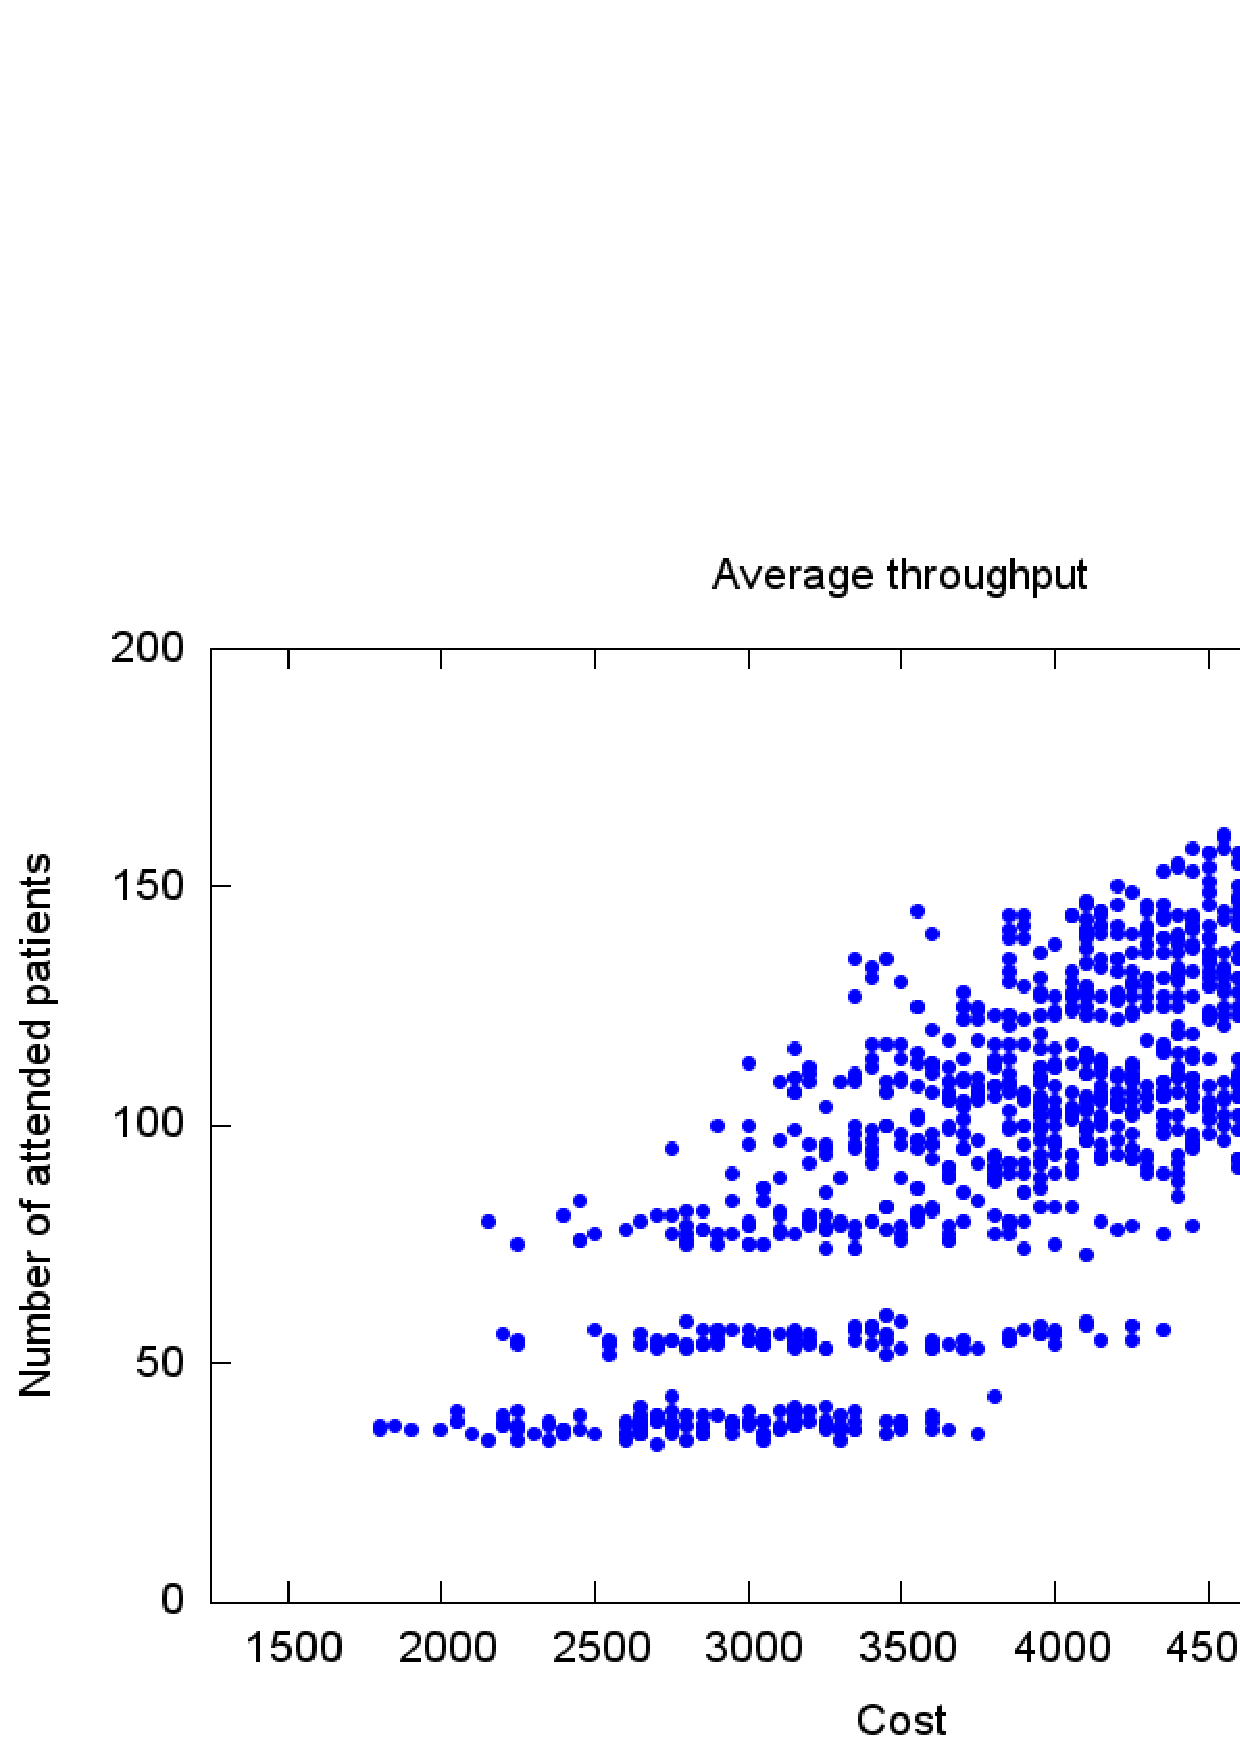
\includegraphics[width=1\columnwidth,height=0.19\paperheight]{figs4/v1\lyxdot 2/MC-518400-23445-100-69-25-1225confs-Throughput}\caption{Average number of attended patients of 1,225 configurations obtained
by the MC method.\label{subfig:mc16-5}}
\end{figure}
\begin{figure}[H]
\begin{centering}
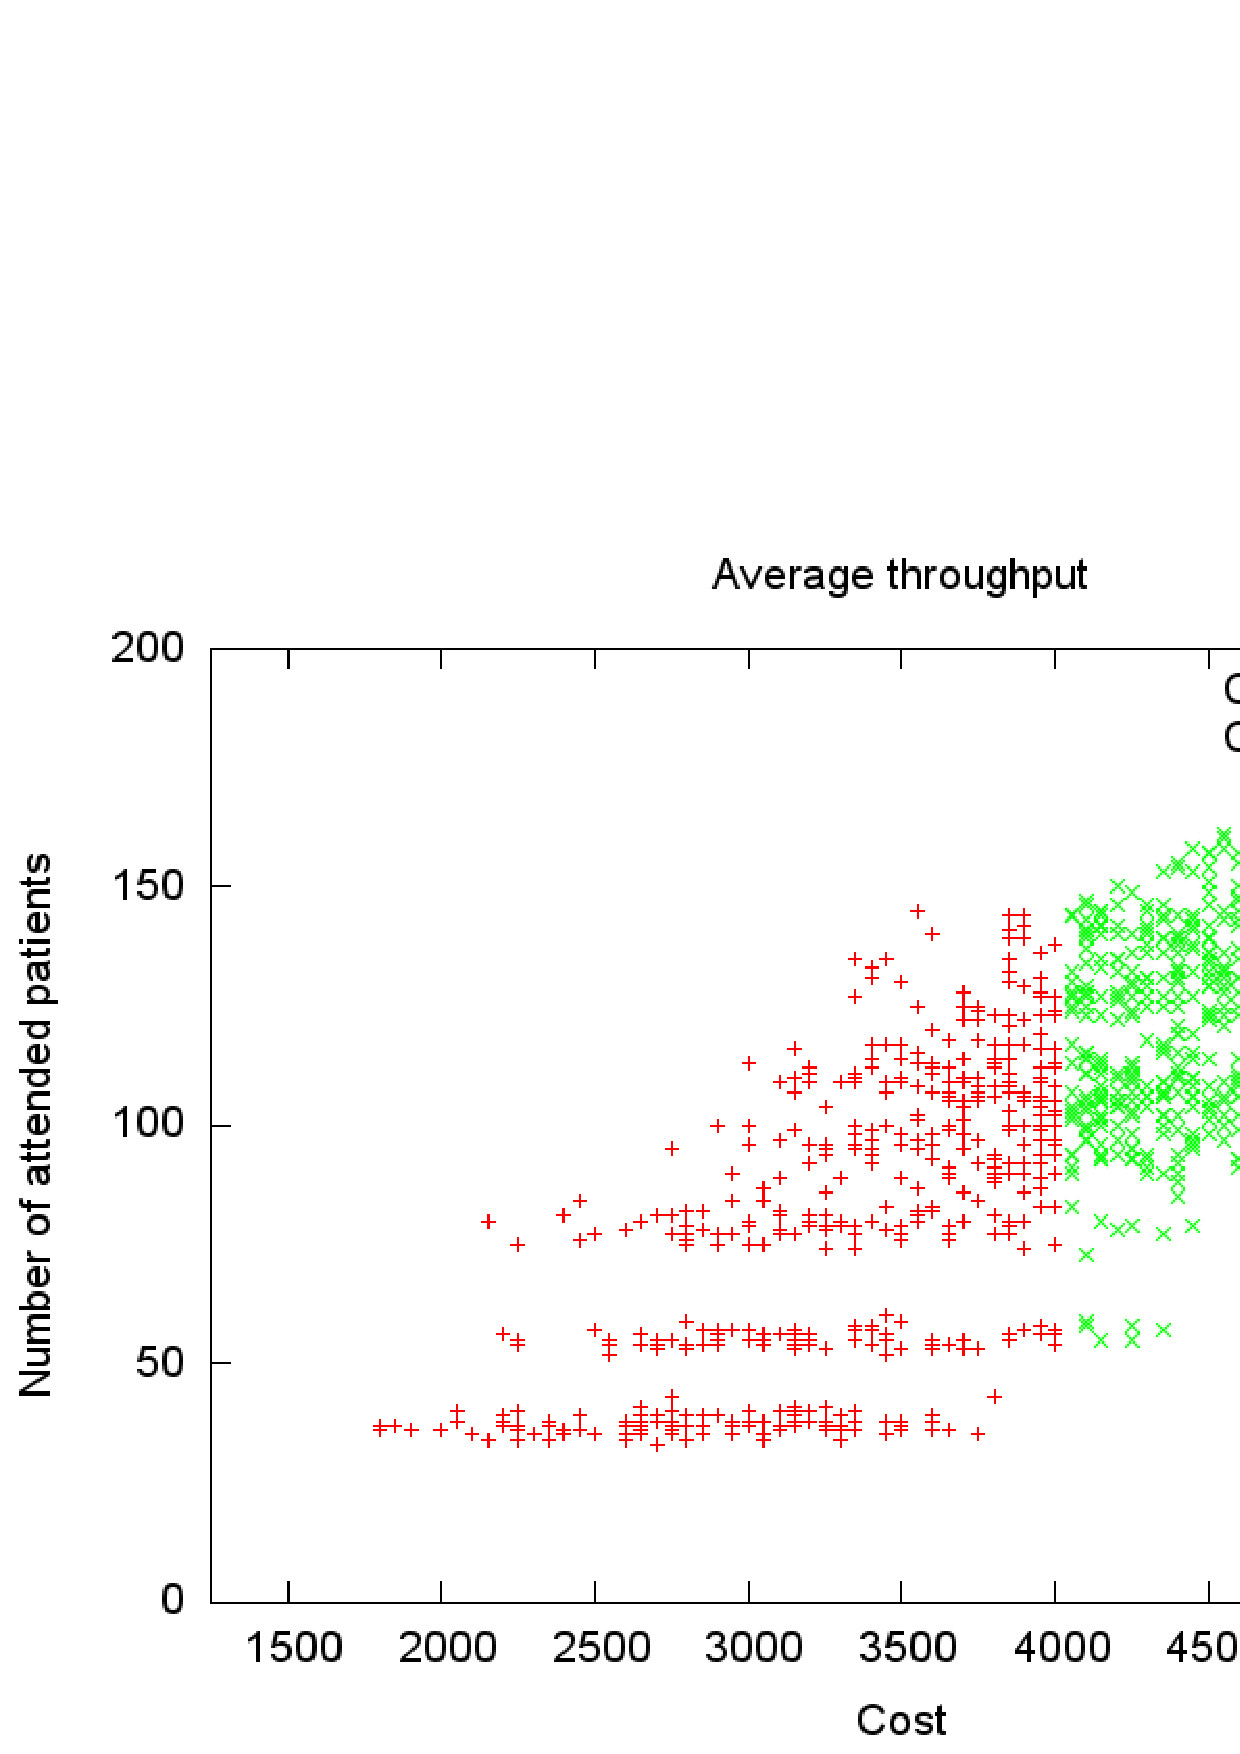
\includegraphics[width=1\columnwidth,height=0.19\paperheight]{figs4/v1\lyxdot 2/K-means-518400-23445-100-69-25-1225-Cluster1-508_Cluster2-688}
\par\end{centering}

\caption{The K-means method identified two clusters of average number of attended
patients. The green one delimited the region where the maximum was.\label{subfig:km16-5}}
\end{figure}


\begin{comment}
The graphics \ref{subfloat:pipe4} and \ref{subfloat:contour4} shown
another way to visualise the connectivity characteristic of the reduced
regions found by the AP, and the MC plus the K-means methods. In such
connected reduced regions the ``reduced exhaustive search'' is applied.
The axes of such graphs are the first column of \ref{subtab:As-pipe},
\ref{subtab:Ns-pipe}, and \ref{subtab:Ds-pipe}, where they were
ordered by the pipeline approach (PA) \ref{eq:Pipeline formula}.
\end{comment}
\begin{comment}
\begin{figure}[H]
\noindent \begin{centering}
\begin{minipage}[t]{0.45\linewidth}%
\noindent \begin{center}
\includegraphics[width=1\columnwidth]{figs4/v1.2/v1-100-exh-throughput-max.png}
\par\end{center}

\noindent \begin{center}
\caption{}

\par\end{center}%
\end{minipage}
\par\end{centering}

\noindent \begin{centering}
\vfill{}

\par\end{centering}

\begin{minipage}[t]{0.45\textwidth}%
\noindent \begin{center}
\includegraphics[width=1\columnwidth]{figs4/v1.2/MC-518400-23445-100-69-25-1225confs-Throughput.png}
\par\end{center}

\caption{}
%
\end{minipage}\hfill{}%
\begin{minipage}[t]{0.45\textwidth}%
\noindent \begin{center}
\includegraphics[width=1\columnwidth]{figs4/v1.2/K-means-518400-23445-100-69-25-1225-Cluster1-508_Cluster2-688.png}
\par\end{center}

\caption{}
%
\end{minipage}
\end{figure}
\end{comment}


Finally, after applied the MC plus the K-means methods, the \textquotedblleft{}reduced
exhaustive search\textquotedblright{} was performed in such reduced
region identified. The optimum found per each method: the ES and the
MC plus the K-means methods are presented in \ref{tab:16p-e}, where
the sanitary staff configuration (doctors, triage nurses, emergency
nurses, x-ray technicians, and admission personnel), their associated
average maximum Throughput, and cost configuration are shown. The
two optima independently found were the same.

\begin{table}[H]
\caption{Optimum staff configurations that got the average maximum Throughput
for this workload scenario (up to 17 patients hourly), where S is
Senior and J is Junior. These optimum sanitary staff configurations
are shown in red triangle in \ref{subfig:es16-5}.}


\begin{centering}
\begin{tabular}{cc>{\centering}p{1.8cm}ccccc>{\centering}p{2.8cm}}
\hline 
Method & � & \#attended patients & D & N & A & EN & XR & Run time (hrs)

256 Pthreads)\tabularnewline
\hline 
ES & 5,400 & 190 & 3S,1J & 1S,1J & 2S,1J & 1J & 1J & 4.41\tabularnewline
MC+K-means & 5,400 & 190 & 3S,1J & 1S,1J & 2S,1J & 1J & 1J & 0.68\tabularnewline
\hline 
\end{tabular}
\par\end{centering}

\label{tab:16p-e} 
\end{table}



\subsection{CLoS Index}

This objective set was to minimise a compound index: $Cost\times LoS$,
(CLoS) in the ED, without any restriction, except the minimum and
maximum number of admission personnel, nurses, doctors, emergency
nurses, and x-ray technicians stated in \Cref{subtab:As-pipe,subtab:Ns-pipe,subtab:Ds-pipe,subtab:ENs-pipe,subtab:XRs-pipe}%
\begin{comment}
\Cref{subtab:As,subtab:Ns,subtab:Ds,subtab:ENs,subtab:Xrs}
\end{comment}
. This index is expressed mathematically in \ref{eq:CLoS index-2}:

\begin{equation}
\begin{aligned} & {\text{Minimise }CLoS} &  & f(D,N,A,En,Xr)\end{aligned}
\label{eq:CLoS index-2}
\end{equation}


As a consequence of not having any constraint, 28,350 ($14D*9N*9A*5En*5Xr$)
staff configurations, that represent the whole search space, were
tested for each of the four workload scenarios of incoming patients
stated in \ref{tab:scenarios}. Because this is a five dimensional
problem, the results are only shown in the following Tables, but the
results maintain the same structure as above case studies.


\subsubsection{First Workload Scenario}

The optimum found per each method: the ES and the MC plus the K-means
methods, after applied the \textquotedblleft{}reduced exhaustive search\textquotedblright{}
in the promising region identified, are presented in \ref{tab:4p-f},
where the sanitary staff configuration (doctors, triage nurses, admission
personnel, emergency nurses, and x-ray technicians), their associated
average minimum CLoS, and cost configuration are shown. The two optimum
independently found were the same. 

\begin{table}[H]
\caption{Optimum staff configurations that got the average minimum CLoS for
this workload scenario (up to 4 patients hourly), where S is Senior
and J is Junior.}


\begin{centering}
\begin{tabular}{cccccccc>{\centering}p{2.8cm}}
\hline 
Method & � & CLoS & D & N & A & EN & XR & Run time (hrs)

256 Pthreads)\tabularnewline
\hline 
ES & 2,050 & $1.02{}^{7}$ & 2S & 1J & 1J & 1J & 1S & 3.73\tabularnewline
MC+K-means & 2,050 & $1.02{}^{7}$ & 2S & 1J & 1J & 1J & 1S & 1.08\tabularnewline
\hline 
\end{tabular}
\par\end{centering}

\label{tab:4p-f}
\end{table}



\subsubsection{Second Workload Scenario}

The optimum found per each method: the ES and the MC plus the K-means
methods, after applied the \textquotedblleft{}reduced exhaustive search\textquotedblright{}
in the promising region identified, are presented in \ref{tab:8p-f},
where the sanitary staff configuration (doctors, triage nurses, admission
personnel, emergency nurses, and x-ray technicians), their associated
average minimum CLoS, and cost configuration are shown. The two optimum
independently found were the same. 

\begin{table}[H]
\caption{Optimum staff configurations that got the average minimum CLoS for
this workload scenario (up to 9 patients hourly), where S is Senior
and J is Junior.}


\begin{centering}
\begin{tabular}{cccccccc>{\centering}p{2.8cm}}
\hline 
Method & � & CLoS & D & N & A & EN & XR & Run time (hrs)

256 Pthreads)\tabularnewline
\hline 
ES & 3,550 & $1.32{}^{7}$ & 4J & 2J & 1S & 1S & 1J & 4.35\tabularnewline
MC+K-means & 3,550 & $1.32{}^{7}$ & 4J & 2J & 1S & 1S & 1J & 2.2\tabularnewline
\hline 
\end{tabular}
\par\end{centering}

\label{tab:8p-f}
\end{table}



\subsubsection{Third Workload Scenario}

The optimum found per each method: the ES and the MC plus the K-means
methods, after applied the \textquotedblleft{}reduced exhaustive search\textquotedblright{}
in the promising region identified, are presented in \ref{tab:12p-f},
where the sanitary staff configuration (doctors, triage nurses, admission
personnel, emergency nurses, and x-ray technicians), their associated
average minimum CLoS, and cost configuration are shown. The two optimum
independently found were the same. 

\begin{table}[H]
\caption{Optimum staff configurations that got the average minimum CLoS for
this workload scenario (up to 13 patients hourly), where S is Senior
and J is Junior.}


\begin{centering}
\begin{tabular}{cccccccc>{\centering}p{2.8cm}}
\hline 
Method & � & CLoS & D & N & A & EN & XR & Run time (hrs)

256 Pthreads)\tabularnewline
\hline 
ES & 1,500 & $1.37{}^{7}$ & 1J & 1J & 1J & 1J & 1J & 5.1\tabularnewline
MC+K-means & 1,500 & $1.37{}^{7}$ & 1J & 1J & 1J & 1J & 1J & 2.7\tabularnewline
\hline 
\end{tabular}
\par\end{centering}

\label{tab:12p-f}
\end{table}



\subsubsection{Fourth Workload Scenario}

The optimum found per each method: the ES and the MC plus the K-means
methods, after applied the \textquotedblleft{}reduced exhaustive search\textquotedblright{}
in the promising region identified, are presented in \ref{tab:16p-f},
where the sanitary staff configuration (doctors, triage nurses, admission
personnel, emergency nurses, and x-ray technicians), their associated
average minimum CLoS, and cost configuration are shown. The two optimum
independently found were the same. 
\begin{table}[H]
\caption{Optimum staff configurations that got the average minimum CLoS for
this workload scenario (up to 17 patients hourly), where S is Senior
and J is Junior.}


\begin{centering}
\begin{tabular}{cccccccc>{\centering}p{2.8cm}}
\hline 
Method & � & CLoS & D & N & A & EN & XR & Run time (hrs)

256 Pthreads)\tabularnewline
\hline 
ES & 1,500 & $1.45{}^{7}$ & 1J & 1J & 1J & 1J & 1J & 5.98\tabularnewline
MC+K-means & 1,500 & $1.45{}^{7}$ & 1J & 1J & 1J & 1J & 1J & 3.03\tabularnewline
\hline 
\end{tabular}
\par\end{centering}

\label{tab:16p-f}
\end{table}


\clearpage{}

\begin{comment}

\section{Performance}

So far, only all the experiments and their results have been presented,
but not the execution time of each experiment. All the execution times
are presented in \ref{exe_time}. It had an execution time of 480
secs., per one case. So, approximately 604 hrs. must be needed, in
order to run the 4,536 staff configuration cases.

\begin{figure}[h]
\includegraphics[width=0.9\columnwidth]{figs4/performance.png}

\caption{}
\end{figure}


\begin{table}[h]
\caption{Execution time.}


\resizebox{4.5in}{!}{ %
\begin{tabular}{|c|c|c|c|c|c|}
\hline 
\multicolumn{1}{|l|}{\textbf{Patients per hour}} & \textbf{4}  & \textbf{9}  & \textbf{13}  & \textbf{17} & \textbf{Problem size} \tabularnewline
\hline 
\textbf{divided by patient arrival (4 cases)}  & 1.03 hrs.  & 2.19 hrs.  & 4.55 hrs.  & \textbf{8.06 hrs}  & 4,536 \tabularnewline
\hline 
\textbf{ parametric approach, split configurations ( 4 cases )}  & 0.19 hrs  & 0.63 hrs.  & 1.5 hrs.  & \textbf{2.7 hrs}  & 4,536 \tabularnewline
\hline 
\textbf{ parametric approach, split configurations ( 32 cases )}  & \multicolumn{1}{l|}{} & \multicolumn{1}{l|}{} & \multicolumn{1}{l|}{} & \textbf{13.01 hrs}  & 28,350 \tabularnewline
\hline 
\end{tabular}} \label{exe_time} 
\end{table}
\end{comment}
\begin{comment}
In the first case, where the search space was divided by the patient
arrival, 4 independent runs were gotten. The best only last almost
an hour, but the worst last almost eight hours. For the second approach,
the search space was divided by both the patient arrival, and the
staff configurations, 64 independent runs, and for the same problem
size it last 4 times less than the previous one. However, there are
clearly imbalance cases, in both experiments, since the running for
4, 9, and 13 patients per hour have quite short execution times. The
last experiment was run only for one case of patient arrival, 17 per
hour, the worst case, it had an execution time of thirteen hours using
64 independent runs.

These quite small configurations of an \emph{ED} demand a lot of time
to simulate and optimise only one day, without doing statistical sensitivity
analysis. The bigger and the more detail an \emph{ED} is, the longer
the execution time is.
\end{comment}
Before finishing this chapter, it is worth reminding that one of the
aims of this research is to help ED managers in setting up strategies
and management guidelines to enhance the performance of such critical
system, as a core member of a DSS. Therefore, we must be aware not
only in finding the optimum solution, but also the sort of such optimum.
Recovering from the first index of case study A: LoS for up to 4 incoming
patient and up to 17 incoming patients shown in \ref{fig:pareto-25}
and \ref{fig:pareto-100}. In \ref{fig:pareto-25} there were plenty
of sanitary staff configurations nearby where the optimum were (inside
the red ellipse). Thus, a sub-optimum solution would be a good solution,
because choosing a sanitary staff configuration cheaper than the optimum
the LoS is approximately the same.

\begin{figure}[H]
\noindent \begin{centering}
\includegraphics[width=0.95\columnwidth,height=0.19\paperheight]{figs4/v0/LoS-Opt-25-pareto}\caption{Average LoS for 4 incoming patients. The red triangle was the minimum.
\label{fig:pareto-25}}

\par\end{centering}

\end{figure}


On the other hand, when there were up to 17 incoming patients in \ref{fig:pareto-100},
it is important to carefully choose the optimum, because there were
not many solutions nearby the optimum (inside the red ellipse), and
selecting a sub-optimum solution would increase the LoS. 
\begin{figure}[H]
\noindent \centering{}\includegraphics[width=0.95\columnwidth,height=0.19\paperheight]{figs4/v0/LoS-Opt-100-pareto}\caption{Average LoS for 17 incoming patients. The red triangle was the minimum.
\label{fig:pareto-100}}
\end{figure}


\clearpage{}


\section{Discussion}

The most relevant conclusions of this chapter are the following:
\begin{enumerate}
\item The two-phase optimisation via simulation of healthcare Emergency
Departments proposed was applied to analyse the administrative strategies
leading to optimum decisions about the physical and human resources
of an ED. In particular, the impact on the economics and the productivity
of Sabadell Hospital ED of different sanitary staff configuration
(v.gr., doctors, triage nurses, admission personnel, emergency nurses,
and x-ray technicians) were analysed.\\

\item The evaluation of the proposal included the \textit{simulation models};
the \textit{decision variables} and\textit{ workloads} used as inputs
of the simulation models; as well as the \textit{metrics} used to
asses the benefits of the proposal. This metrics were defined in term
of three indexes: patient length of stay (LoS) in the ED; number of
attended patients per day (Throughput); and a compound index, the
product of the cost of a given sanitary staff configuration times
patient length of stay (CLoS).\\

\item From interviews with the managers at the EDs of Sabadell hospital
(which provides healthcare services to an average of 160,000 patients/year),
it was found that a basic sanitary of its ED staff is composed by:
9 possible combinations of admission personnel (junior/senior); 9
possible combinations of triage nurses (junior/senior); 5 possible
combinations of emergency nurses (junior/senior); 5 possible combinations
of x-ray technicians (junior/senior); and 14 possible combinations
of doctors (junior/senior) in which a set of examined cases for each
type of staff were analysed as a discrete combinatorial problem.\\

\item In order to analyse the performance of the ED, the real average four
hundred incoming patients that daily arrive to the ED of Sabadell
hospital was divided into four different workload scenarios, up to:
4, 9, 13, and 17 incoming patients hourly, i.e., up to 96, 216, 312,
and 408, respectively for 24hrs.\\

\item All simulations of the ED optimization cases analysed in this work
were carried out in a Linux cluster of the CAOS Department of the
UAB, which has 608 computing cores and 2.2TB of RAM, that is composed
of: 9 nodes of a dual-4 core Intel Xeon E5430, 2.6GHz, 16GB RAM; 1
node of 2xdual-6 core Intel Xeon E5645, 2.4GHz, 24GB RAM; and 8 nodes
of 4x16-cores AMD Opteron ``Interlagos'', 1.66GHz, 256 GB RAM, all
in a switched 1GigE network.\\

\item The evaluation of the proposed methodology aimed to confirm the correct
operation of both the pipeline approach (PA) and the MC plus the K-means
methods, described in \ref{chap3:Math}. To this end, we have first
performed the exhaustive search (ES) to use as baseline method. The
second step of this evaluation consisted on applying the coarse grained
phase, using either the PA, the MC plus K-means methods, or both.
Finally, the fine grained phase was applied in the promising regions
found in the previous step.\\

\item To evaluate the methodology proposed, first the case study A was performed
using the agent-based ED simulator version 1.1. Then the case study
B was performed using the agent-based ED simulator version 1.2. In
both cases, the three metrics and the four different workloads stated
above were tested, and the period simulated was 24 hrs., i.e., one
day of functioning of the ED, in all the experiments.\\

\item After separately applying for cases A and B either the pipeline approach,
PA or the Monte Carlo, MC, plus the K-means methods, or both the \textquotedblleft{}reduced
exhaustive search\textquotedblright{}, the optimum found per each
method for their associated average LoS, average Throughput, and average
CLoS were the same.\\

\item Using the pipeline approach, PA, as the coarse grained phase of the
proposed methodology and then the \textquotedblleft{}reduced exhaustive
search\textquotedblright{} in the promising regions previously found,
our proposal obtained an improvement up to 95.6\% in the computing
time, whereas using the Monte Carlo, MC, plus the K-means methods
and then the \textquotedblleft{}reduced exhaustive search\textquotedblright{}
in the promising regions previously found, our proposal obtained an
improvement up to 72\% in the computing time, both compared with the
exhaustive search used.
\item The optimum solution not always is the best option; it is important
to take into account the sort of optimum when the solutions are going
to be applied into real problems or decision support systems.
\end{enumerate}

\end{document}
